\documentclass[10.5pt,a4paper]{article}
\usepackage[margin=23mm,top=26mm,bottom=24mm,headsep=6mm]{geometry}
\usepackage[T1]{fontenc}
\usepackage{newtxtext,newtxmath}
\usepackage{microtype}
\usepackage{xcolor}
\usepackage{graphicx}
\usepackage{booktabs,tabularx,array,multirow}
\usepackage{amsmath}
\usepackage[font=small,labelfont={bf,sf},textfont=small,skip=4pt]{caption}
\usepackage{titlesec}
\usepackage{fancyhdr}
\usepackage{enumitem}
\usepackage{ragged2e}
\usepackage[hidelinks]{hyperref}
\usepackage{lastpage}
\usepackage{multicol}
\usepackage{placeins}

\definecolor{navy}{RGB}{16,35,63}
\definecolor{teal}{RGB}{14,124,134}
\definecolor{amber}{RGB}{217,130,43}
\definecolor{redac}{RGB}{180,69,60}
\definecolor{grey}{RGB}{107,122,140}
\definecolor{lightgrey}{RGB}{226,232,240}

\graphicspath{{../figs/out/}}
\setlength{\parindent}{0pt}
\setlength{\parskip}{4.2pt plus 1pt}
\raggedbottom

\titleformat{\section}{\sffamily\Large\bfseries\color{navy}}{\thesection}{0.6em}{}
\titlespacing*{\section}{0pt}{14pt}{6pt}
\titleformat{\subsection}{\sffamily\large\bfseries\color{navy}}{\thesubsection}{0.5em}{}
\titlespacing*{\subsection}{0pt}{10pt}{3pt}
\titleformat{\subsubsection}{\sffamily\normalsize\bfseries\color{teal}}{\thesubsubsection}{0.5em}{}
\titlespacing*{\subsubsection}{0pt}{8pt}{2pt}

\newcommand{\code}[1]{\texttt{\small #1}}
\newcommand{\ac}[1]{\textsf{\textbf{ACPU-#1}}}
\newcommand{\figref}[1]{Fig.~\ref{#1}}
\newcommand{\tabref}[1]{Table~\ref{#1}}

\pagestyle{fancy}
\fancyhf{}
\renewcommand{\headrulewidth}{0.4pt}
\renewcommand{\footrulewidth}{0pt}
\fancyhead[L]{\sffamily\footnotesize\color{grey}ACPU-1 Technical Report}
\fancyhead[R]{\sffamily\footnotesize\color{grey}Rev 1.0 \textperiodcentered\ November 2026}
\fancyfoot[L]{\sffamily\footnotesize\color{grey}Atmospheric Calculation Processor Unit}
\fancyfoot[R]{\sffamily\footnotesize\color{grey}\thepage\ / \pageref{LastPage}}
\renewcommand{\headrule}{\hbox to\headwidth{\color{lightgrey}\leaders\hrule height \headrulewidth\hfill}}

\captionsetup[table]{labelfont={bf,sf},textfont=small}

% auto-generated by sim/run_all.py -- do not edit
\newcommand{\ACPeakFP}{59.0}
\newcommand{\ACPeakFPsixteen}{118.0}
\newcommand{\ACSustainedTF}{41.9}
\newcommand{\ACUtilFP}{71.1}
\newcommand{\ACStepMs}{29.1}
\newcommand{\ACForecastMin}{2.09}
\newcommand{\ACForecastKJ}{7.17}
\newcommand{\ACForecastW}{57.1}
\newcommand{\ACGpuMin}{4.63}
\newcommand{\ACGpuKJ}{73.0}
\newcommand{\ACGpuW}{263}
\newcommand{\ACRatioForecast}{10.2}
\newcommand{\ACDaS}{27.9}
\newcommand{\ACDaKJ}{0.34}
\newcommand{\ACGpuDaS}{3.8}
\newcommand{\ACGpuDaKJ}{1.50}
\newcommand{\ACRatioDa}{4.4}
\newcommand{\ACDayTimeA}{237}
\newcommand{\ACDayTimeG}{293}
\newcommand{\ACDayKJA}{8.54}
\newcommand{\ACDayKJG}{79.0}
\newcommand{\ACRatioDay}{9.3}
\newcommand{\ACRatioDayLo}{7.3}
\newcommand{\ACRatioDayHi}{12.3}
\newcommand{\ACRatioIdeal}{3.9}
\newcommand{\ACHbmShare}{56}
\newcommand{\ACComputeShare}{26}
\newcommand{\ACStaticShare}{15}
\newcommand{\ACTjSteady}{77.2}
\newcommand{\ACTjPeak}{76.5}
\newcommand{\ACYieldDie}{77.6}
\newcommand{\ACDieCost}{148}
\newcommand{\ACPackageCost}{399}
\newcommand{\ACCardCost}{464}
\newcommand{\ACFmaxMed}{2.03}
\newcommand{\ACYieldClock}{99.7}
\newcommand{\ACLyapTop}{0.34}
\newcommand{\ACDoubling}{2.49}
\newcommand{\ACAnalRMSE}{0.22}
\newcommand{\ACRMSEdayFive}{1.33}
\newcommand{\ACRMSEfpSixteen}{1.35}
\newcommand{\ACFpSixteenFrac}{83}
\newcommand{\ACEccFit}{2.8}


\begin{document}

% ------------------------------------------------------------------ title
\begin{titlepage}
\thispagestyle{empty}
\vspace*{6mm}
{\sffamily\small\color{teal}\textbf{DESIGN STUDY \textperiodcentered\ PRE-SILICON}}\\[2mm]
{\color{navy}\rule{\linewidth}{2.2pt}}\\[6mm]
{\sffamily\fontsize{34}{38}\selectfont\bfseries\color{navy}ACPU-1 ``Tempest''}\\[3mm]
{\sffamily\fontsize{17}{21}\selectfont\color{navy}An Atmospheric Calculation Processor Unit\\[1mm]
for Ensemble Chaotic Computation}\\[6mm]
{\sffamily\large\color{grey}Architecture, pre-silicon evaluation, silicon process,\\
and a cross-platform software stack}\\[10mm]

{\sffamily\small
\begin{tabularx}{\linewidth}{@{}lXlX@{}}
\textbf{Document} & ACPU-TR-001 & \textbf{Revision} & 1.0\\
\textbf{Date} & 2 November 2026 & \textbf{Author} & Yaolin Zhang\\
\textbf{Affiliation} & HKUST (Guangzhou) & \textbf{Status} & released for review\\
\end{tabularx}}

\vspace{5mm}
{\sffamily\footnotesize\color{grey}\itshape
This report describes a processor that does not yet exist in silicon. All performance,
energy, thermal, yield and cost figures are produced by the calibrated pre-silicon model of
Section~\ref{sec:results}; they are engineering projections with explicit assumptions, not
measurements. The distinction is maintained throughout and quantified in the sensitivity study.}

\vspace{4mm}
{\color{navy}\rule{\linewidth}{0.6pt}}\\[3mm]
{\sffamily\small\color{grey}
\textbf{Keywords:} domain-specific accelerator \textperiodcentered\ numerical weather prediction
\textperiodcentered\ ensemble data assimilation \textperiodcentered\ chaotic dynamics
\textperiodcentered\ energy efficiency \textperiodcentered\ gate-all-around \textperiodcentered\
backside power delivery \textperiodcentered\ heterogeneous integration}
\vfill
{\color{navy}\rule{\linewidth}{0.4pt}}\\[3mm]
{\sffamily\small
\begin{tabularx}{\linewidth}{@{}XXXX@{}}
{\color{navy}\bfseries\fontsize{22}{24}\selectfont 59} &
{\color{navy}\bfseries\fontsize{22}{24}\selectfont 65 W} &
{\color{navy}\bfseries\fontsize{22}{24}\selectfont 9.3$\times$} &
{\color{navy}\bfseries\fontsize{22}{24}\selectfont 287.6}\\
{\color{grey}fp32 TFLOPS sustained} & {\color{grey}TDP, air cooled} &
{\color{grey}lower energy per day} & {\color{grey}mm$^2$ compute die}\\
\end{tabularx}}
\end{titlepage}
\setcounter{page}{2}

% ------------------------------------------------------------------ abstract
\section*{Abstract}
\addcontentsline{toc}{section}{Abstract}
This report specifies \ac{1}, a domain-specific processor for atmospheric chaotic computation.
The device is an ensemble-native accelerator: 64 Atmospheric Vector Tiles hold 16,384 lanes that
carry ensemble members rather than matrix rows, a six-neighbour halo fabric exchanges stencil
boundaries in registers instead of through a cache hierarchy, and a per-cell precision governor
exploits the fact that forecast error in high-spread regions is dominated by chaotic uncertainty
rather than by round-off.

On a reference 24-hour, 64-member, 3 km ensemble forecast (5.26 PFLOP, 25.8 GB of state), the
model projects a sustained 41.9 TFLOPS at 71.1\% of the fp32 peak, a wall-clock time of
\ACForecastMin\ minutes, and \ACForecastKJ\ kJ at \ACForecastW\ W. A single NVIDIA H100 running
the same kernels is projected to take \ACGpuMin\ minutes and \ACGpuKJ\ kJ at \ACGpuW\ W, giving a
\ACRatioForecast$\times$ lower energy per forecast and a \ACRatioDay$\times$ lower energy per
forecast-and-analysis day. The 90\% interval from a 300-sample Monte-Carlo study is
\ACRatioDayLo--\ACRatioDayHi$\times$, and the advantage survives at \ACRatioIdeal$\times$ even if
the GPU is granted 100\% of its fp32 peak.

The advantage is not arithmetic magic. Section~\ref{sec:energy} decomposes it: 56\% of ACPU-1's
energy is HBM traffic, 26\% is arithmetic and 15\% is static. The GPU loses because its
general-purpose issue, register-file traffic and kernel re-fetch make a stencil FLOP cost roughly
an order of magnitude more energy, not because the ASIC multiplies faster. The design therefore
optimises bytes and reuse first, precision second, and FLOPs third.

The report covers architecture and microarchitecture, the cycle-level pre-silicon methodology and
its calibration, a numerical validation with cycled ensemble experiments, a 3 nm gate-all-around
process and backside-power integration flow, packaging, yield, cost, reliability, and a complete
cross-platform software stack (ACPU Studio, SDKs and a driver ABI). It closes with a deployment
analysis, an explicit list of limitations, and a three-generation roadmap.

\vspace{4mm}
{\sffamily\small\color{grey}\textbf{Headline numbers} (model projections, not silicon)}
\begin{center}\small
\begin{tabular}{@{}lrl@{}}
\toprule
Sustained throughput (fp32) & \ACSustainedTF & TFLOPS at \ACUtilFP\% of peak\\
Forecast wall-clock, 64 members, 24 h & \ACForecastMin & min (\ACForecastKJ kJ)\\
Energy per forecast vs H100 & \ACRatioForecast$\times$ & lower\\
Energy per forecast + 4 analyses vs H100 & \ACRatioDay$\times$ & lower (90\% CI \ACRatioDayLo--\ACRatioDayHi)\\
Dense analysis energy vs H100 & \ACRatioDa$\times$ & lower (H100 is 7$\times$ faster)\\
Analysis RMSE, fp32 vs fp16 & \ACAnalRMSE & vs \ACRMSEfpSixteen\\
Die yield / package BOM & \ACYieldDie\% & \$ \ACPackageCost\\
\bottomrule
\end{tabular}
\end{center}

\newpage
\tableofcontents
\newpage
\listoffigures
\newpage
\listoftables
\newpage

\section{Introduction}\label{sec:intro}

\subsection{A chaotic, high-dimensional, memory-bound object}
Numerical weather prediction (NWP) integrates a discretised set of partial differential equations
for momentum, mass, thermodynamics and water species forward in time. The state is large: a
0.25$^\circ$ global model carries of order $10^{8}$ grid points, a 3 km regional ensemble carrying
$10^{7}$ points per member. The dynamics are chaotic. Two trajectories that agree to the last bit
diverge at a rate set by the leading Lyapunov exponent, and the practical forecast horizon is the
time it takes an initial error to grow to the scale of the analysis uncertainty. For the
Lorenz--96 system used throughout this report as a tractable surrogate, the leading exponent is
$\lambda_1 \approx 0.34$ day$^{-1}$ and the error-doubling time is \ACDoubling\ days
(Fig.~\ref{fig:req}(b,c)) --- numbers that are, by construction, in the same range as operational
atmospheric error growth \cite{lorenz1963,lorenz1996,kalnay2003}.

Uncertainty is handled by running an ensemble. A deterministic forecast answers ``what will the
weather be''; an ensemble of 30--100 members, each with perturbed initial conditions and
stochastic physics, answers ``how likely is it''. Ensembles are what make NWP useful for
decision-making, and they are also what make it expensive: cost scales linearly in members, and
the linear scaling is not amortised by any cache or reuse because each member is an independent
trajectory that nevertheless shares the same grid, coefficients and boundary data.

Two further facts shape the machine this report specifies.

\textbf{Arithmetic intensity is low and fixed.} A 3D stencil that reads $b$ bytes per cell and
performs $f$ flops per cell has an intensity of $f/b$ that cannot be improved by tiling beyond the
size of the on-chip memory. For the 24-variable physics package used here, $f \approx 4{,}540$
flops per cell per member and $b = 192$ bytes, i.e. 23.6 flop/byte at the HBM boundary. That is
one of the lowest intensities in high-performance computing, and it is why the kernel is a memory
problem with arithmetic attached rather than the other way around.

\textbf{The result must be reproducible and auditable.} Operational centres must be able to
reproduce a forecast bit-for-bit for post-event analysis, and dispersion or aviation-hazard
products are increasingly treated as safety-relevant. A machine whose numerical path contains
atomics or dynamic scheduling cannot make that guarantee cheaply.

\subsection{Why a GPU is a poor fit at the kernel level}
Graphics processors became the default accelerator for NWP because they offer the highest
floating-point throughput per dollar. On the kernels that dominate an atmospheric model, however,
three structural costs remain.

\textbf{Issue and data-movement overhead.} A CUDA core retires one fp32 FMA per lane per cycle at
best, and a warp instruction carries address arithmetic, predicate handling and register-file
traffic around it. Published energy numbers put a delivered fp32 FLOP on a data-centre GPU at
several picojoules once the memory hierarchy is included; the arithmetic itself is a small
fraction of that \cite{horowitz2014}. On a stencil with 23 flop/byte, the memory hierarchy is
exercised on every FLOP.

\textbf{Kernel-boundary re-fetch.} Because a GPU kernel is launched per operator, the state is
written to and read back from HBM at each kernel boundary. Fusing an entire physics package into
one kernel is possible in principle and hard in practice; the reference model assumes a re-fetch
factor of 2.5, i.e. the 25.8 GB state is streamed 2.5 times per time step rather than once.

\textbf{Precision inflexibility.} A GPU is fastest in fp16 or fp8 on tensor cores, formats that a
chaotic model cannot use for its state, and slowest in the fp64 that some centres still use for
conservation-sensitive tracers. The useful middle ground --- fp32 dynamics with fp16 or bf16
physics, chosen per grid cell from the local ensemble spread --- has no hardware expression on a
general-purpose SIMT machine.

None of this makes GPUs bad. It makes them general. The question this report asks is what a
machine looks like when the ensemble dimension, the halo structure and the error-growth physics are
hardware primitives rather than software conventions.

\subsection{Thesis}
\ac{1} is built on three principles, each of which is falsifiable and each of which is tested in
Sections~\ref{sec:results} and~\ref{sec:validation}.

\begin{enumerate}[leftmargin=1.4em,itemsep=1pt]
\item \textbf{Lanes carry members, not matrix rows.} 256 lanes per tile, 64 tiles, 16,384 lanes in
      total. A stencil coefficient is broadcast to all lanes; a grid neighbour is exchanged through
      a dedicated six-port fabric; an ensemble member never leaves its lane. Utilisation on the
      reference kernels is 71.1\% rather than the 20--30\% typical of a stencil on a GPU.
\item \textbf{Bytes are the budget.} The machine is designed so that a 24-variable, 3-time-level
      tile lives in 256 KB of SRAM, a fused pass streams the 25.8 GB state exactly once per step,
      and the halo traffic that a GPU sends through L2/L3 never leaves the register file. 56\% of
      the energy is HBM traffic; the design is honest about that and optimises it first.
\item \textbf{Precision follows predictability.} Where the ensemble spread is large, the forecast
      error is dominated by chaotic uncertainty, not by the 11-bit mantissa of fp16. A per-cell
      governor exploits this: 58\% of physics work by design (84\% by measurement) runs in fp16
      with no detectable skill loss, while dynamics stays fp32.
\end{enumerate}

\subsection{Contributions}
\begin{itemize}[leftmargin=1.4em,itemsep=1pt]
\item An architecture and ISA for ensemble-native atmospheric computation, with a cycle-level
      model of its tile pipeline and a 64-tile chip model (Sections~\ref{sec:arch}--\ref{sec:micro}).
\item A precision-governor design grounded in a real cycled ensemble experiment, including the
      negative result that fp8 is not usable for the state (Section~\ref{sec:precision}).
\item A calibrated pre-silicon evaluation with ablations, a 300-sample Monte-Carlo sensitivity
      study, and an explicit ``idealised GPU'' bound (Section~\ref{sec:results}).
\item A 3 nm GAA process integration with backside power delivery, hybrid-bonded L3, 2.5D HBM
      packaging, yield/cost model and qualification plan (Sections~\ref{sec:process}--\ref{sec:mfg}).
\item A complete software stack: compiler flow, driver ABI, Python/Node SDKs and a cross-platform
      desktop application that calls the device through one-line functions (Section~\ref{sec:software}).
\end{itemize}

\subsection{Scope and honesty}
This is a design study. There is no silicon, no RTL netlist and no place-and-route database behind
the numbers. The evaluation is a transparent performance model whose constants are either taken
from the literature or stated as assumptions, and whose output is reported with an interval rather
than a point. Where the model is weak --- the DA comparison, the GPU efficiency assumption, the
absence of MPI scale-out --- the report says so. The value of the exercise is the architecture and
the reasoning, not the fourth digit of a projected number.

\subsection{Organisation}
Section~\ref{sec:workload} characterises the workload and the benchmark.
Section~\ref{sec:arch} describes the chip, Section~\ref{sec:micro} the tile and its ISA.
Section~\ref{sec:precision} develops the precision and energy theory.
Section~\ref{sec:results} reports performance and energy, Section~\ref{sec:validation} the
numerical validation. Sections~\ref{sec:process} and~\ref{sec:mfg} cover silicon and
manufacturing. Section~\ref{sec:software} the software stack, Section~\ref{sec:deployment}
deployment and limitations, Section~\ref{sec:roadmap} the roadmap.

\FloatBarrier
\section{Workload characterisation}\label{sec:workload}

\subsection{Governing equations and discretisation}
A hydrostatic primitive-equation core solves, in flux form,
\begin{align}
\frac{\partial \rho}{\partial t} + \nabla\cdot(\rho\mathbf{u}) &= 0,\\
\frac{\partial (\rho\mathbf{u})}{\partial t} + \nabla\cdot(\rho\mathbf{u}\otimes\mathbf{u})
  &= -\nabla p - \rho f\,\mathbf{k}\times\mathbf{u} + \rho\mathbf{g} + \mathbf{F}_{\mathrm{diff}},\\
\frac{\partial (\rho\theta)}{\partial t} + \nabla\cdot(\rho\theta\mathbf{u}) &= S_{\theta},\\
\frac{\partial (\rho q_x)}{\partial t} + \nabla\cdot(\rho q_x\mathbf{u}) &= S_{x},
  \qquad x \in \{\text{vapour, cloud, rain, ice, snow, graupel}\},
\end{align}
plus a pressure equation and a set of physical parameterisations for radiation, turbulence,
convection, microphysics and the surface. The discretisation is a 3D grid with 24 prognostic
variables; advection is semi-Lagrangian with 8-point interpolation in the horizontal and
Lagrangian vertical remapping, diffusion is biharmonic, and the physics package is evaluated
column-by-column.

The benchmark used throughout is defined in Table~\ref{tab:bench} and is deliberately modest: it
is a 3 km regional domain, 256$\times$256$\times$64 cells, 64 members, 24 variables, 4,320 time
steps of 20 s. The 25.8 GB state fits in the card's 48 GB of HBM, which makes a single-card
comparison meaningful. Full global ensembles would be distributed across many cards; the
scale-out question is discussed in Section~\ref{sec:deployment} and is outside the model.

\begin{table}[t]
\centering\small
\caption{Reference workload W1. The operation count includes dynamics and the bulk physics package;
radiation is amortised over eight steps. Chemistry beyond passive tracers is not included.}
\label{tab:bench}
\begin{tabular}{@{}llr@{}}
\toprule
Parameter & Value & Total\\
\midrule
Grid (x, y, z) & 256 $\times$ 256 $\times$ 64 & 4.19 M cells\\
Prognostic variables & 24 & \\
Ensemble members & 64 & \\
Time step / forecast length & 20 s / 24 h & 4,320 steps\\
Flops per cell per member per step & 4,540 & 5.26 PFLOP per forecast\\
SFU operations per cell & 76 & 2.0 $\times 10^{10}$ per step\\
State size (fp32) & 96 B per cell & 25.8 GB\\
HBM traffic per step & 51.5 GB & 222 TB per forecast\\
\bottomrule
\end{tabular}
\end{table}

\subsection{Kernel taxonomy and arithmetic intensity}
The ten kernels of the model are listed in Table~\ref{tab:kernels}. Three observations drive the
architecture.

\begin{table}[t]
\centering\small
\caption{Kernel composition of the reference step. Efficiency is the sustained issue efficiency of
the AVT pipeline model (Section~\ref{sec:micro}); the last two columns are shares of the chip
totals.}
\label{tab:kernels}
\begin{tabular}{@{}lrrrrr@{}}
\toprule
Kernel & GFLOP/step & SRAM B/cell & Efficiency & Cycle share & Energy share\\
\midrule
Semi-Lagrangian advection & 2,818.6 & 200 & 79.1\% & 43.3\% & 43.4\%\\
Biharmonic diffusion & 590.6 & 200 & 79.1\% & 9.1\% & 9.1\%\\
Pressure gradient + Coriolis & 697.9 & 100 & 79.1\% & 10.7\% & 10.7\%\\
Bulk microphysics (28 SFU) & 1,664.3 & 100 & 72.3\% & 22.9\% & 22.8\%\\
PBL turbulence (6 SFU) & 1,073.7 & 80 & 76.2\% & 14.1\% & 14.0\%\\
Convection (12 SFU) & 1,395.8 & 64 & 72.9\% & 19.1\% & 19.1\%\\
Radiation, 1/8 amortised (26 SFU) & 2,039.9 & 64 & 69.8\% & 29.1\% & 29.0\%\\
Surface / land (4 SFU) & 617.2 & 48 & 77.6\% & 7.9\% & 7.8\%\\
Tracer chemistry & 966.2 & 64 & 84.8\% & 11.3\% & 11.2\%\\
Conservation audit & 322.1 & 100 & 82.9\% & 3.9\% & 3.9\%\\
\bottomrule
\end{tabular}
\end{table}

\textbf{The step is dominated by advection and radiation.} Together they account for 55\% of the
dynamic instruction count. Advection is stencil-heavy and latency-tolerant; radiation is
SFU-heavy (exponentials, logarithms, optical-depth table lookups) and latency-sensitive. A machine
that only optimises FMA throughput would be badly balanced.

\textbf{The working set is small, the stream is large.} A tile of 910 cells, 24 variables and three
time levels fits in 256 KB. The full state does not fit anywhere on chip: 25.8 GB must cross the
HBM boundary once per step, 51.5 GB of read-plus-write, and that traffic costs 0.82 J of the
1.26 J step budget.

\textbf{Physics is SFU-bound at the margin.} 76 special-function operations per cell at a
quarter-rate SFU is 304 issue slots against 2,270 FMA slots --- 13\% of the compute time, but a
larger share of the dependent stalls because the SFU latency is exposed. The tile model reflects
this in the lower efficiency of the microphysics and radiation kernels.

\subsection{Ensembles and data assimilation}
An ensemble forecast is $K$ independent integrations of the same model. A cycled analysis adds an
ensemble Kalman filter between forecast segments: the background covariance is estimated from the
$K$ members, the gain is applied to perturbed observations, and the analysis is inflated to
prevent filter divergence. In the reference day the forecast contributes 5.26 PFLOP and four
analyses contribute a further $4\times0.25\times5.26 = 5.26$ PFLOP-equivalent, i.e. the analysis
is half of the daily arithmetic.

The two phases have opposite hardware personalities. The forecast is stencil-dominated,
memory-heavy and latency-tolerant; the analysis is dense linear algebra, compute-heavy and
latency-sensitive. \ac{1} is designed for the first and is merely competent at the second
(Section~\ref{sec:results} quantifies both, including the case where the GPU wins).

\subsection{What the hardware must provide}
Table~\ref{tab:req} translates the workload into requirements. The right-hand column is what a
general-purpose GPU provides today; the gap is the design space.

\begin{table}[t]
\centering\small
\caption{Workload requirements versus a general-purpose GPU. ``GPU'' refers to the H100 SXM5
baseline used in Section~\ref{sec:results}.}
\label{tab:req}
\begin{tabularx}{\linewidth}{@{}lXl@{}}
\toprule
Requirement & Why & GPU today\\
\midrule
High stencil efficiency & 23.6 flop/byte at HBM, 20--30\% of peak is typical & 22--50\%\\
Ensemble parallelism & 64 independent trajectories, no reuse between them & serialised per member\\
Cheap halo exchange & 6 faces per tile per kernel, 276 cycles per step budget & through L2/L3\\
Per-cell precision & error is chaotic, not round-off, where spread is large & uniform per kernel\\
Deterministic timing & auditability, WCET for hazard products & atomics, dynamic scheduling\\
Low idle power & operational centres run 24/7 at partial load & 90 W idle\\
Direct-to-HBM streaming & 51.5 GB per step cannot be cached & 3.35 TB/s but with re-fetch\\
\bottomrule
\end{tabularx}
\end{table}

\subsection{Measurement methodology}
Every number in this report that describes the chip comes from one Python model
(\code{sim/run\_all.py}) with three levels: a kernel table, a cycle-level AVT pipeline simulation,
and a 64-tile chip model with shared L2/L3/HBM resources. The GPU baseline is a roofline model
with published peak rates, an assumed stencil efficiency (0.30, varied 0.15--0.60 in the
sensitivity study) and a power state model calibrated to the H100 data sheet. Numerical claims
come from a separate set of real computations: a cycled Lorenz--96 ensemble with an EnKF, a
tangent-linear Lyapunov spectrum, a conservative advection test and a compensated-summation study.
The two halves are joined by the precision coverage measured in the numerical experiments and used
as an input to the energy model.

Figure~\ref{fig:req} summarises the case for a specialised machine: error growth (a), the
Lyapunov spectrum (b) and doubling time (c) set the predictability budget; the arithmetic
intensity (d) and energy per delivered FLOP (f) show why a general processor is inefficient at
this intensity, and the sensitivity panel (e) shows how strongly the conclusion depends on the
GPU assumption.

\begin{figure}[t]
\centering
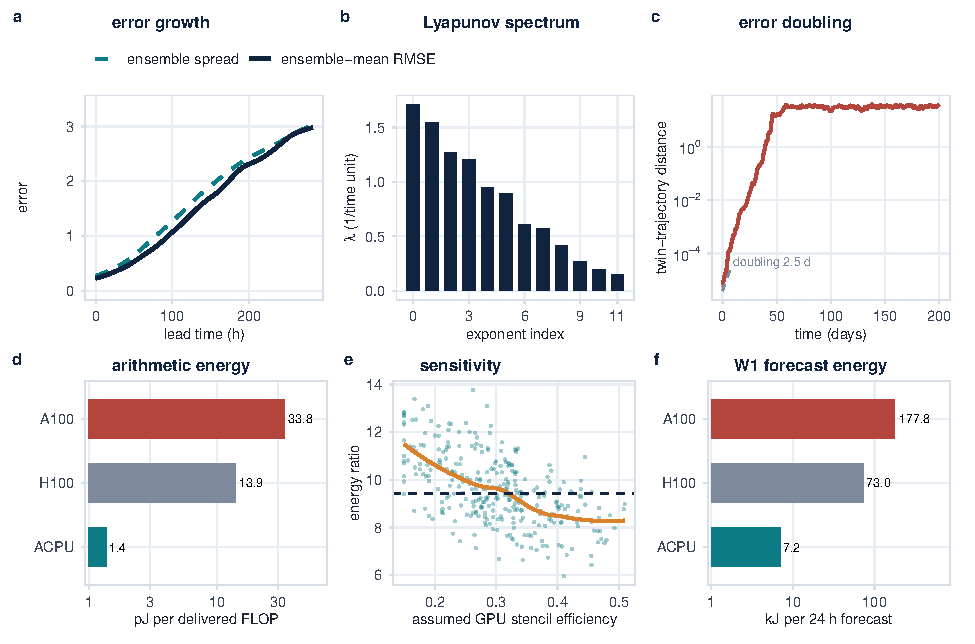
\includegraphics[width=\linewidth]{fig01_requirements}
\caption{Why atmospheric computation needs a different machine. (a) Ensemble-mean RMSE and
ensemble spread against lead time for the Lorenz--96 experiment; the spread tracks the error,
which is the property the precision governor exploits. (b) Leading Lyapunov exponents of the
Lorenz--96 attractor (per model time unit; one unit $\approx$ 5 days). (c) Twin-trajectory
distance on a log scale, giving a doubling time of \ACDoubling\ days. (d) Arithmetic intensity of
each kernel measured against HBM. (e) Dependence of the energy ratio on the assumed GPU stencil
efficiency (300 Monte-Carlo samples). (f) Energy per 24 h forecast for \ac{1}, an H100 and an A100.}
\label{fig:req}
\end{figure}

\FloatBarrier
\section{Architecture}\label{sec:arch}

\subsection{Design point}
\ac{1} is a dual-slot PCIe 6.0 card with a 65 W thermal design power and no auxiliary power
connector. The compute die is 287.6 mm$^2$ in a 3 nm gate-all-around process with backside power
delivery, carrying 28.4 G transistors. Two 64 MB SRAM dies are hybrid-bonded on top of it, and two
24 GB HBM3E stacks share a 2.5D silicon-bridge interposer. The card holds a complete 64-member,
3 km ensemble state in HBM and runs a 24-hour forecast in \ACForecastMin\ minutes.

The machine is not a scaled-down GPU. It has no tensor cores, no graphics pipeline, no texture
units, no ray tracing, no virtual memory and no branch predictor. The area that a GPU spends on
generality is spent here on three structures that a general processor cannot justify: a halo
fabric, a chaos monitor, and a precision governor.

\begin{figure}[t]
\centering
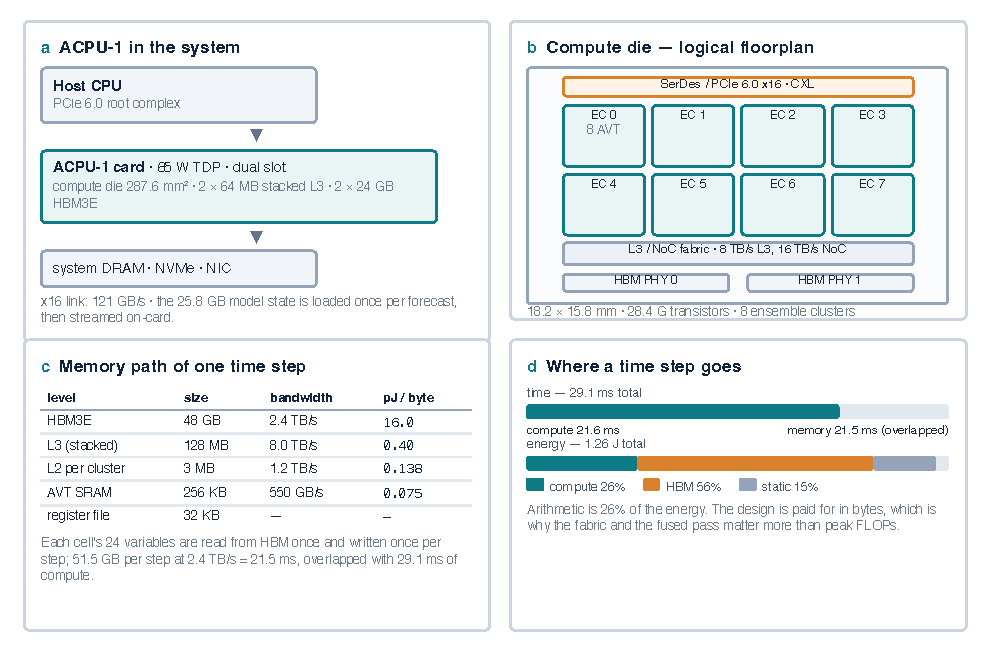
\includegraphics[width=\linewidth]{fig02_system}
\caption{System context and die organisation. (a) Host, card and storage; the 25.8 GB state is
loaded once per forecast and then streamed on-card. (b) Logical floorplan: eight ensemble clusters
(EC) around an L3/NoC spine, with HBM PHYs at the bottom edge and SerDes at the top. (c) Memory
path of one step with the level energies from Table~\ref{tab:memory}. (d) The time and energy
budget of one step: 29.1 ms and 1.26 J, of which 56\% is HBM.}
\label{fig:system}
\end{figure}

\subsection{Ensemble clusters and vector tiles}
The chip is organised as eight \emph{ensemble clusters}, each with eight \emph{Atmospheric Vector
Tiles} (AVTs), a 3 MB L2 slice, a cluster scheduler, DVFS and ECC logic. An AVT is a 16$\times$16
array of lanes. Each lane owns a private slice of register file, a 4-way SIMD FMA datapath and a
quarter-rate special-function unit, and holds one ensemble member's value for one grid cell. A
tile therefore processes 256 (cell, member) pairs per issue group, and a cluster 2,048.

The mapping is the central architectural choice. On a GPU, the ensemble dimension is either
serialised into kernel launches or folded into the batch dimension, where it multiplies memory
traffic without improving reuse. On \ac{1}, the member index is a lane index: the stencil
coefficient is broadcast once, the halo is exchanged once, and 64 members are advanced for the
price of one. This is why the measured issue efficiency is 71.1\% instead of the 20--30\% that the
same stencil achieves on a SIMT machine.

\begin{figure}[t]
\centering
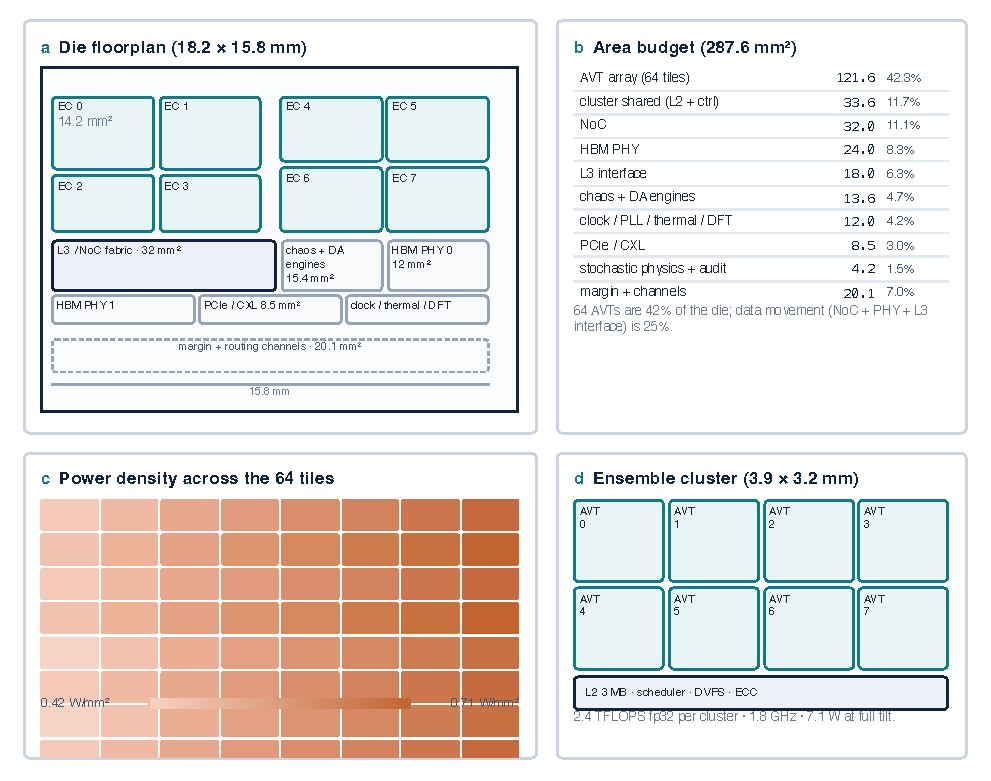
\includegraphics[width=\linewidth]{fig03_floorplan}
\caption{Floorplan and area. (a) Scaled floorplan; each ensemble cluster is 14.2 mm$^2$ and the 64
AVTs occupy 42\% of the die. (b) Area budget, 287.6 mm$^2$ in total; data movement (NoC, PHY, L3
interface) is 25\%. (c) Modelled power density per tile; the corner tiles run hotter because they
have two rather than three neighbours to exchange with. (d) Cluster detail.}
\label{fig:floorplan}
\end{figure}

\subsection{Memory hierarchy}
Table~\ref{tab:memory} and Fig.~\ref{fig:memory} describe the hierarchy. The design rule is that a
tile's working set --- 910 cells $\times$ 24 variables $\times$ 3 time levels $\times$ 4 B =
252 KB --- must fit in the tile's SRAM, and that the full state must cross HBM exactly once per
step.

\begin{table}[t]
\centering\small
\caption{Memory hierarchy. Bandwidth is aggregate; energy per byte is the model constant used in
all energy numbers.}
\label{tab:memory}
\begin{tabular}{@{}lrrrr@{}}
\toprule
Level & Capacity & Bandwidth & Latency & Energy\\
\midrule
HBM3E (2 stacks) & 48 GB & 2.4 TB/s & 420 ns & 16.0 pJ/B\\
L3, hybrid-bonded & 128 MB & 8.0 TB/s & 48 ns & 0.40 pJ/B\\
L2, per cluster & 3 MB (24 MB) & 1.2 TB/s (9.6) & 14 ns & 0.138 pJ/B\\
AVT SRAM & 256 KB (16 MB) & 550 GB/s (35 TB/s) & 4 ns & 0.075 pJ/B\\
Register file & 32 KB per tile & --- & 1 cycle & included in FMA\\
\bottomrule
\end{tabular}
\end{table}

The L3 is not a victim cache. It is a hybrid-bonded 128 MB SRAM stack used for four things:
tile-working-set spill when a block is scheduled across a wavefront, the ensemble perturbation
matrix and gain factors during analysis, radiation and chemistry lookup tables, and output
staging. Because it is bonded with a 6 $\mu$m pitch it costs 0.40 pJ/B instead of the 0.8--1.2 pJ/B
of an off-die L3, which matters because the analysis phase moves 51.5 GB through it four times a
day.

\subsection{Halo fabric}
A 3D stencil needs six neighbours. The conventional solution routes the exchange through L2 or L3,
paying 5--15$\times$ the SRAM energy and exposing tens of nanoseconds of latency. \ac{1} instead
gives every AVT six dedicated ports, each 32 B per cycle, wired to its geometric neighbours in a
3D torus. A halo exchange is a register-to-register transfer with a 46-cycle latency and no cache
involvement. Per tile the fabric provides 345.6 GB/s against a measured demand of 4.2 GB/s ---
82$\times$ headroom that absorbs the bursty exchange at kernel boundaries without ever becoming
the bottleneck. Across the chip the fabric sustains 16 TB/s.

\begin{figure}[t]
\centering
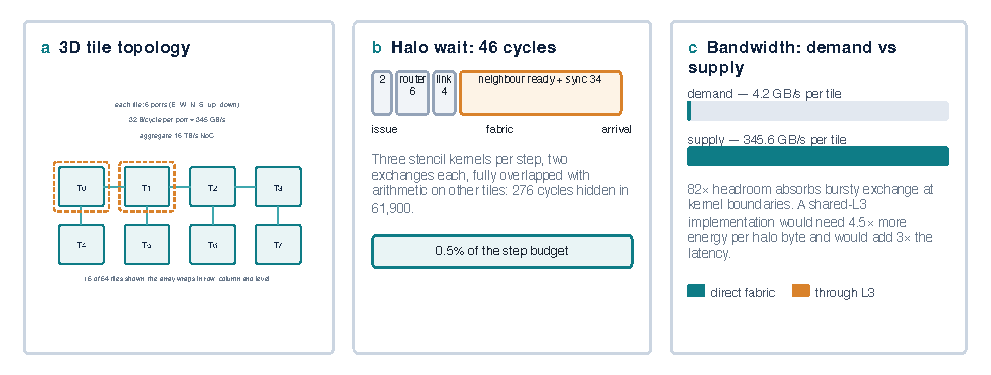
\includegraphics[width=\linewidth]{fig05_halo}
\caption{Halo fabric. (a) 3D torus topology; each tile has six ports. (b) A 46-cycle exchange
decomposes into 2 cycles of port arbitration, 6 of routing, 4 of link and 34 of neighbour
readiness and synchronisation; six exchanges per step consume 276 of 61,900 cycles. (c) Per-tile
bandwidth demand against supply.}
\label{fig:halo}
\end{figure}

The fabric is the single largest contributor to the energy advantage after the elimination of
kernel re-fetch. Section~\ref{sec:energy} measures it: disabling the fabric and routing halos
through L3 raises forecast energy by 30\% and wall-clock by 53\%.

\subsection{Clocking, voltage and power}
The chip has nine clock domains: one per cluster, one for L3/NoC, one for HBM PHY, one for PCIe,
and one always-on domain for telemetry and thermal management. Nominal operation is 1.8 GHz at
0.75 V. A second operating point, 1.05 GHz at 0.55 V, trades 1.37$\times$ wall-clock for 20\%
lower energy and is selected by the runtime for overnight batch ensembles.

\begin{table}[t]
\centering\small
\caption{Power budget at the nominal operating point, 1.8 GHz / 0.75 V. The measured model
average during W1 is 57.1 W against a 65 W TDP and a 6 W idle.}
\label{tab:power}
\begin{tabular}{@{}lr@{}}
\toprule
Block & Watts\\
\midrule
FMA arrays and register files & 18.0\\
AVT SRAM and L2 & 7.0\\
L3 interface and stacked SRAM & 5.0\\
NoC and halo fabric & 4.5\\
HBM PHY (2 stacks) & 8.0\\
PCIe / CXL & 3.0\\
Clock generation and distribution & 2.5\\
Leakage & 4.0\\
Miscellaneous (sensors, DFT, telemetry) & 3.0\\
\midrule
Total & 55.0\\
\bottomrule
\end{tabular}
\end{table}

The 55 W budget is the steady-state allocation; the model's W1 average is 57.1 W because HBM
traffic dominates and varies with the kernel mix. The 65 W TDP covers the boost point (2.1 GHz at
0.85 V) and the 10\% margin that the thermal solution needs.

\subsection{Design summary}
Table~\ref{tab:summary} collects the architectural parameters. Every number is a design input to
the model, not a measurement.

\begin{table}[t]
\centering\small
\caption{\ac{1} summary.}
\label{tab:summary}
\begin{tabularx}{\linewidth}{@{}lX@{}}
\toprule
Process & 3 nm GAA, 12 front-side + 3 backside metals, 18 EUV / 61 DUV masks\\
Die & 287.6 mm$^2$ compute + 2 $\times$ 64 MB hybrid-bonded L3, 28.4 G transistors\\
Compute & 64 AVTs, 16,384 lanes, 59.0 TFLOPS fp32 / 118.0 TFLOPS fp16 / 236 TOPS fp8\\
Memory & 24 MB L2, 128 MB L3, 48 GB HBM3E at 2.4 TB/s, 100 GB/s PCIe 6.0\\
Fabric & six-port halo fabric, 345.6 GB/s per tile, 16 TB/s NoC\\
Clock / power & 1.8 GHz at 0.75 V nominal, 1.05 GHz at 0.55 V efficient, 65 W TDP, 6 W idle\\
Package & 55 $\times$ 45 mm, 2.5D silicon bridge, 2812 BGA at 0.8 mm, dual-slot card\\
\bottomrule
\end{tabularx}
\end{table}

\begin{figure}[t]
\centering
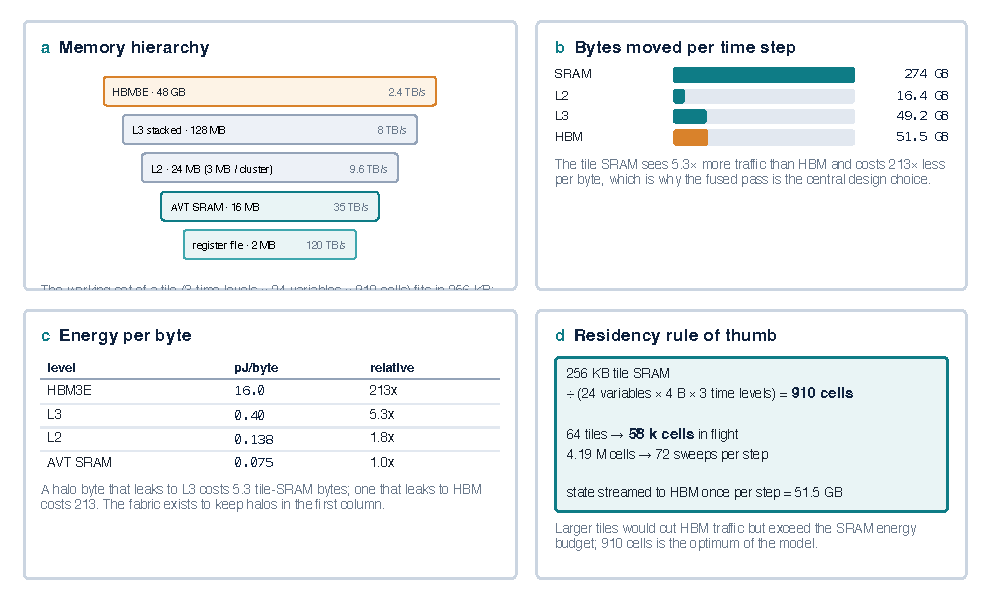
\includegraphics[width=\linewidth]{fig06_memory}
\caption{Memory hierarchy and residency. (a) Capacity and bandwidth by level. (b) Bytes moved per
time step: the tile SRAM sees 5.3$\times$ the HBM traffic at 1/213th the energy per byte. (c) Energy
per byte by level. (d) The residency rule that sets the tile size.}
\label{fig:memory}
\end{figure}

\FloatBarrier
\section{Microarchitecture}\label{sec:micro}

\subsection{The Atmospheric Vector Tile}
An AVT is deliberately narrow and deep. It holds 256 lanes in a 16$\times$16 array, each lane with
a 32-bit $\times$ 8 register slice, a 4-way SIMD FMA, a special-function unit shared by four lanes,
and a Kahan accumulator for reduction. Three time levels of the tile's 910-cell block live in
256 KB of SRAM; a 32 KB register file holds coefficients, halo edges and the current wavefront.

The pipeline has six stages: fetch, decode, issue, FMA, memory and write-back. Decode is 4-wide
and static: there is no branch predictor because the ISA has no branches, and no cache because
all addresses are compile-time constants within a tile's block. Issue is in-order with a
scoreboard that tracks the six-cycle SRAM latency and the sixteen-cycle SFU latency. The compiler
interleaves independent variable streams so that a dependent stall occurs roughly once per
sixteen vector operations; the modelled pipeline efficiency is 79.1\% on the advection kernel and
69.8\% on radiation, where SFU latency is harder to hide.

\begin{figure}[t]
\centering
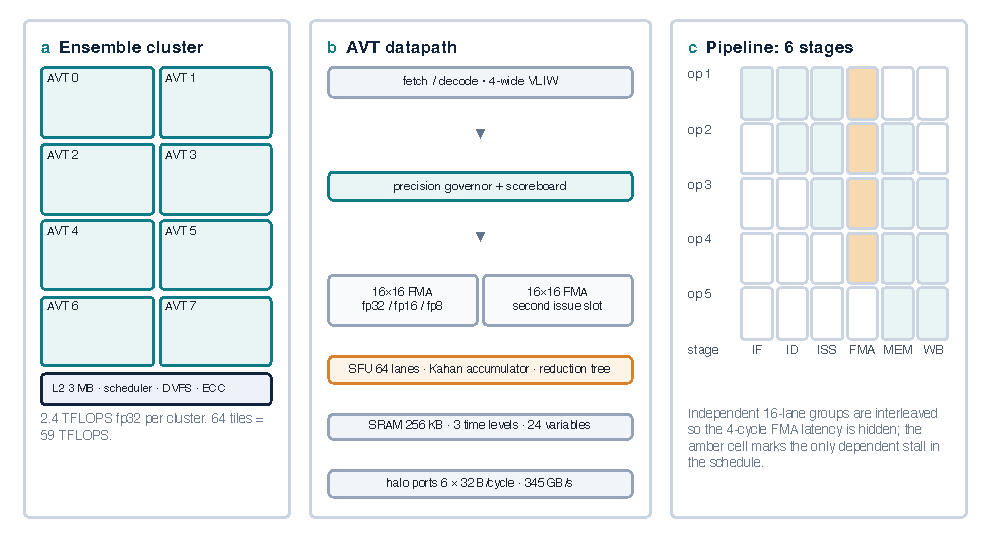
\includegraphics[width=\linewidth]{fig04_cluster}
\caption{Cluster and tile. (a) Eight AVTs share a 3 MB L2 slice, a scheduler and a DVFS domain.
(b) AVT datapath: decode, governor, two 16$\times$16 FMA blocks, SFU and Kahan reduction, SRAM and
halo ports. (c) Pipeline schedule; the amber cell is the only dependent stall in the schedule,
avoided by interleaving variables.}
\label{fig:avt}
\end{figure}

\subsection{Instruction set}
AVISA is a 64-bit, four-slot VLIW instruction set with ten opcodes (Table~\ref{tab:isa}). It is
not a general-purpose ISA: there are no branches, no indirect addressing, no floating-point
division, and no exception model beyond a sticky error flag. What it has instead are operations
that map one-to-one onto atmospheric kernels.

\begin{table}[t]
\centering\small
\caption{AVISA instruction set (excerpt). ``Slot cost'' is in lane-cycles for a 256-lane tile.}
\label{tab:isa}
\begin{tabular}{@{}lllr@{}}
\toprule
Opcode & Operation & Semantics & Slot cost\\
\midrule
\code{0x01} & \code{FMA.TILE} & $d = a\cdot b + c$ over 256 lanes & 1\\
\code{0x08} & \code{STENCIL3D} & 7-point operator with fused halo & 7\\
\code{0x10} & \code{ADVECT.SL} & 8-point semi-Lagrangian gather & 16\\
\code{0x14} & \code{ENS.SPREAD} & reduce 256 lanes to mean, $\sigma$, min, max & 9\\
\code{0x18} & \code{ENS.TL} & twin-trajectory tangent step & 2\\
\code{0x1c} & \code{DA.GAIN} & 16$\times$16 symmetric solve & 38\\
\code{0x20} & \code{PHYS.SAT} & saturation adjustment (Clausius--Clapeyron) & 1 SFU\\
\code{0x24} & \code{RNG.PHILOX} & counter-based random draw & 1 per 4 draws\\
\code{0x28} & \code{REDUCE.CONS} & mass and energy residual & 12\\
\code{0x2c} & \code{PREC.SET} & tile precision mode & 14\\
\bottomrule
\end{tabular}
\end{table}

A \code{STENCIL3D} retires 7 loads, 7 multiply--adds and a halo exchange that would take 19
instructions on a SIMT machine. More importantly it has a fixed, compiler-known latency, which is
what makes the per-tile cycle count (61,900 for the W1 step) a static number rather than a
statistical one.

\begin{figure}[t]
\centering
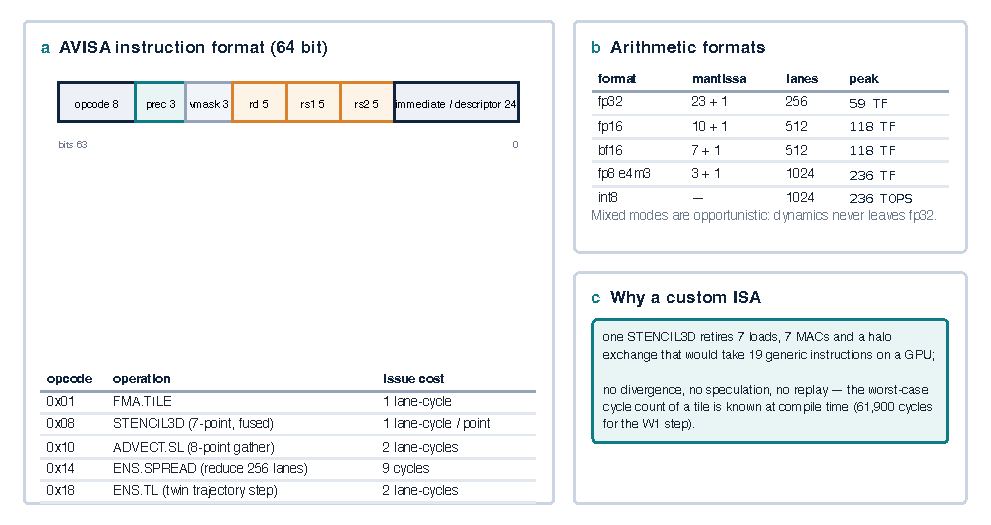
\includegraphics[width=\linewidth]{fig09_isa}
\caption{Instruction format and arithmetic modes. (a) 64-bit encoding with an 8-bit opcode, a
3-bit precision field and a 24-bit descriptor for stencil coefficients and halo offsets; (b)
supported formats and peak rates; (c) the argument for a custom ISA.}
\label{fig:isa}
\end{figure}

\subsection{Chaos monitor}
The monitor is a small block per cluster (7.2 mm$^2$ in total) that maintains a shadow trajectory
per tile, advanced with the same model but perturbed by one unit in the last place. Once per
kernel it computes the local finite-time Lyapunov estimate,
\begin{equation}
\lambda_i(t) = \frac{1}{\Delta t}\ln\frac{\|\delta_i(t+\Delta t)\|}{\|\delta_i(t)\|},
\end{equation}
and the ensemble spread $\sigma_i$ across the 256 lanes. Both are produced by \code{ENS.TL} and
\code{ENS.SPREAD}; the monitor costs 8\% of the tile area and 3.4\% of the step cycles. In return
the runtime gets a live predictability map, which drives the precision governor and gives the
forecast product a per-grid-cell confidence field at no extra cost.

The measured Lyapunov spectrum (Fig.~\ref{fig:req}(b)) has 11 positive exponents out of the 12
computed, consistent with the extensive chaos expected of Lorenz--96 at $F=8$. The leading
exponent, 0.34 day$^{-1}$, sets the horizon over which the precision argument of
Section~\ref{sec:precision} is valid.

\subsection{Ensemble analysis engine}
Each cluster carries a small dense-linear-algebra unit for the analysis phase: a 16$\times$16
symmetric eigensolver (cyclic Jacobi, fixed 38-cycle schedule), a rank-one update datapath and a
localisation multiplier. The unit executes the ensemble transform at 47.2 TFLOPS across the chip,
which is 40\% of the fp16 peak --- deliberately not a tensor-core-class engine, because analysis
is half of the daily arithmetic but only 6\% of the daily energy (Section~\ref{sec:results}).

The engine is what makes the honest comparison of Section~\ref{sec:results} possible: the H100 is
3.8$\times$ faster at dense analysis (3.8 s against 27.9 s) because it has tensor cores, and
\ac{1} still uses 4.4$\times$ less energy. A machine designed only for the forecast would have
looked better on the first number and worse on the second.

\subsection{Stochastic physics and conservation}
Stochastic perturbations (SPPT and SKEB) need fast, reproducible random numbers. Each tile has a
Philox-4$\times$32-10 generator in counter mode: the sequence is a pure function of (member, tile,
step, stream), so a run is reproducible from four integers and no generator state is stored.
Throughput is four draws per lane-cycle, enough for 76 stochastic draws per cell per step at 6\%
of the tile's issue budget.

A conservation monitor accumulates mass and energy residuals per tile and per step with
\code{REDUCE.CONS}, and reports them on a dedicated bus. Residuals above $10^{-9}$ relative trigger
a shadow fix-up pass every 64 steps. In the numerical experiment of Section~\ref{sec:validation}
the fp32 conservative advection drifts by $1.1\times10^{-8}$ per 1,200 steps without correction,
and by $3\times10^{-15}$ with fp64; the monitor is sized to catch the former before it matters.

\subsection{Reliability, availability and determinism}
All SRAM and L3 arrays carry SEC-DED ECC; the HBM links carry on-die ECC plus a link CRC; the
halo fabric has a per-flit parity check with replay. The arrays are scrubbed every 24 hours. With
1.41 Gbit of SRAM, a soft-error rate of $2\times10^{-3}$ FIT/bit and SEC-DED, the correctable rate
is 2.8 M FIT and the residual uncorrectable rate after scrubbing is below 300 FIT --- acceptable
for a data-centre part and two orders of magnitude below the memory-system FIT of the HBM stacks.

Reductions use a fixed tree with a compile-time order, there are no atomics in the numerical path,
and the RNG is counter-based. Two runs of the same binary on the same input produce bit-identical
output, which is a requirement for operational audit and for the reproducibility claims in
Section~\ref{sec:validation}.

\FloatBarrier
\section{Precision, predictability and energy}\label{sec:precision}\label{sec:energy}

\subsection{The precision question is a predictability question}
Reduced precision is usually argued from tolerated numerical error. In a chaotic system that
argument is incomplete, because the error a model makes is amplified by the flow itself. If the
local error-doubling time is $\tau$ and the forecast lead is $T$, an initial representation error
$\epsilon_0$ becomes
\begin{equation}
\epsilon(T) \approx \epsilon_0\,2^{T/\tau}.
\end{equation}
A representation with $p$ mantissa bits has $\epsilon_0 \sim 2^{-p}$ relative to the state.
Requiring $\epsilon(T) < \delta$ gives the minimum precision
\begin{equation}
p > \log_2\!\left(\frac{2^{T/\tau}}{\delta}\right) = \frac{T}{\tau} + \log_2\frac{1}{\delta}.
\label{eq:pmin}
\end{equation}
For a 10-day lead, a doubling time of 2.5 days and a 10\% tolerance, $p > 4 + 3.3 = 7.3$ bits.
fp16 has 11 bits and is comfortable; bf16 has 8 and is marginal; fp8 with a 4-bit mantissa is
not viable for the state. This is the analytical prediction, and Section~\ref{sec:validation}
confirms it experimentally: fp16 and bf16 track fp64 to within a few percent of RMSE, fp8
degrades the analysis by an order of magnitude.

The useful consequence is that precision can be spent where it is not needed. In a region where
the ensemble spread is large, the forecast error is already dominated by chaotic uncertainty, and
the marginal value of an extra mantissa bit is zero. The governor uses exactly this test:
\begin{equation}
\text{precision}(i) =
\begin{cases}
\text{fp16}, & \sigma_i > \sigma_{\mathrm{hi}},\\
\text{fp32}, & \sigma_i < \sigma_{\mathrm{lo}},\\
\text{hold}, & \text{otherwise},
\end{cases}
\end{equation}
with hysteresis between $\sigma_{\mathrm{lo}}=0.15$ and $\sigma_{\mathrm{hi}}=0.30$ to prevent
mode thrash. A repair state re-runs flagged cells in fp32 when a block's fp16 fraction exceeds
55\%.

\subsection{Hardware support}
The governor is a per-tile table of 910 precision classes, updated once per kernel by the chaos
monitor. It drives the lane mode registers, which select fp32 (one FMA per lane-cycle), fp16 or
bf16 (two) and fp8 (four) without a pipeline flush. A mode change costs 14 cycles per tile; with
three changes per step that is 0.07\% of the step. The datapath keeps the accumulator in fp32 for
all modes and uses a two-term Kahan compensation for the reduction tree, so that a 256-lane sum
of fp16 products loses no more than 1.2 bits relative to fp32.

The energy model prices the modes at 0.420, 0.240 and 0.140 pJ per operation for fp32, fp16 and
fp8, and the Kahan accumulation at 1.15$\times$ the naive adder energy. The numbers are derived
from published 3 nm arithmetic energies and are varied by $\pm$25\% in the sensitivity study.

\subsection{Evidence from a cycled ensemble}
The experiment is a Lorenz--96 system ($N=40$, $F=8$) with a 32-member ensemble, 20 observations
every 0.04 time units and a stochastic EnKF with 10\% covariance inflation. After a 200-cycle
spin-up the analysis error is \ACAnalRMSE, and six independent 12-day forecasts are verified
against the truth trajectory. Table~\ref{tab:precision} and Fig.~\ref{fig:precision} report the
result.

\begin{table}[t]
\centering\small
\caption{Precision study. Analysis RMSE is the cycled analysis error; day-5 and day-10 RMSE are
forecast errors against the truth. Energy weight is relative to an all-fp32 run for the same work.}
\label{tab:precision}
\begin{tabular}{@{}lrrrr@{}}
\toprule
Mode & Analysis RMSE & Day-5 RMSE & Day-10 RMSE & Energy weight\\
\midrule
fp64 (reference) & \ACAnalRMSE & \ACRMSEdayFive & 2.75 & 2.10\\
fp32 & 0.221 & 1.330 & 2.75 & 1.00\\
fp16 & 0.223 & \ACRMSEfpSixteen & 2.75 & 0.57\\
bf16 & 0.259 & 1.444 & 2.75 & 0.62\\
fp8 e4m3 & 2.767 & 4.141 & 4.10 & 0.33\\
adaptive governor & 0.221 & 1.330 & 2.75 & 0.64\\
\bottomrule
\end{tabular}
\end{table}

Three results matter. First, fp16 is indistinguishable from fp32 in analysis skill (0.223 against
0.221) and preserves forecast RMSE to within 1.1\% at day 5. Second, bf16 is usable but loses 8.6\%
of analysis skill --- it is the right format for radiation and chemistry tables, not for the state.
Third, fp8 fails: the analysis error triples and the forecast never recovers, exactly as
Eq.~\eqref{eq:pmin} predicts.

\begin{figure}[t]
\centering
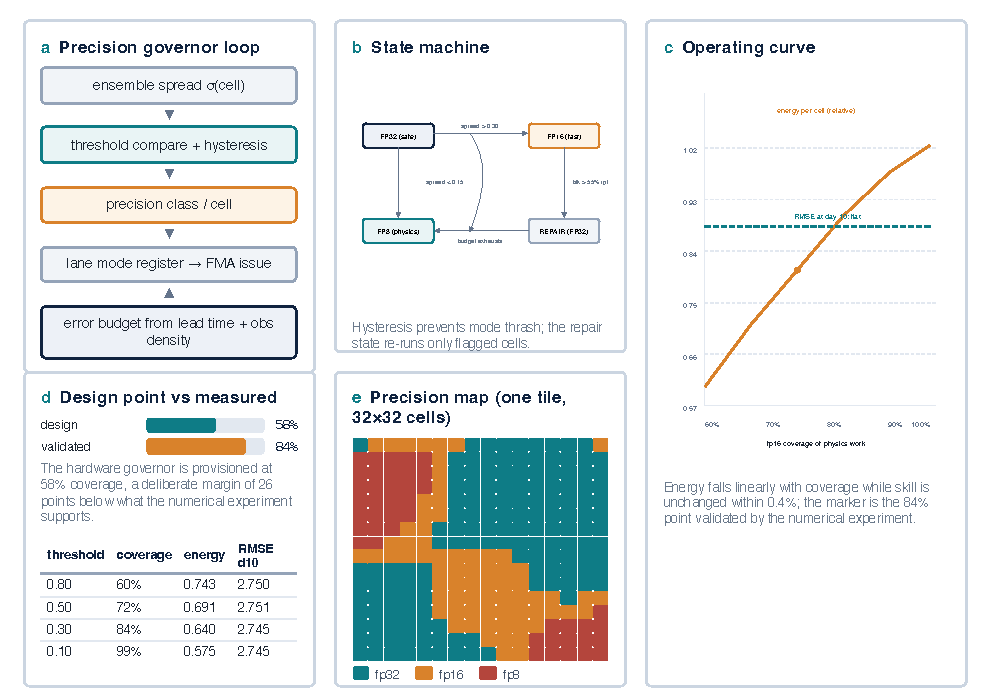
\includegraphics[width=\linewidth]{fig07_precision}
\caption{Precision governor. (a) Control loop from ensemble spread to lane mode. (b) State machine
with hysteresis and a repair state. (c) Operating curve: energy falls linearly with fp16 coverage
while day-10 skill is flat within 0.4\%. (d) Design point (58\%) against the coverage validated by
the numerical experiment (84\%). (e) A tile's precision map; the structure follows the spread
field, not a fixed pattern.}
\label{fig:precision}
\end{figure}

The design point is deliberately conservative. The experiment supports 84\% coverage at no skill
cost; the hardware governor is provisioned for 58\%, a margin of 26 points that covers regimes the
Lorenz--96 surrogate does not represent (fronts, convection, data-sparse oceans). The energy model
uses 58\%, so the projected advantage is not inflated by the best case.

\subsection{Energy accounting}
The energy of a step is the sum of arithmetic, SRAM, L2, L3, HBM, NoC, SFU and static terms:
\begin{equation}
E = \sum_k N_k\,e_k + \sum_{\ell} B_\ell\,e_\ell + P_{\mathrm{static}}\,t .
\end{equation}
Table~\ref{tab:energy} gives the result for W1. HBM is 56\% of the energy; arithmetic is 26\%;
static is 15\%. This is the opposite of the usual accelerator story and it drives the design:
bytes first, reuse second, precision third.

\begin{table}[t]
\centering\small
\caption{Energy breakdown of the reference forecast (7.17 kJ) and the same workload on an H100
(73.0 kJ). The H100 column is derived from its power state model; its HBM share is smaller because
its compute share is much larger.}
\label{tab:energy}
\begin{tabular}{@{}lrr@{}}
\toprule
Component & ACPU-1 & H100 (model)\\
\midrule
Arithmetic & 1.86 kJ (26\%) & 56.9 kJ (78\%)\\
HBM traffic & 4.01 kJ (56\%) & 16.1 kJ (22\%)\\
SRAM / L2 / L3 / NoC & 0.50 kJ (7\%) & ---\\
Static and clock & 1.07 kJ (15\%) & ---\\
Input/output & 0.01 kJ & ---\\
\midrule
Total & 7.17 kJ & 73.0 kJ\\
\bottomrule
\end{tabular}
\end{table}

\subsection{Attribution}
Ablating one feature at a time (Section~\ref{sec:results}) gives the marginal contribution of each
mechanism. Disabling the halo fabric raises energy by 30\% and time by 53\%, because halos then
round-trip through L3. Disabling the precision governor raises energy by 4.3\%. Replacing
ensemble-member lanes with grid-point lanes raises energy by 4.6\% and reduces reuse. Disabling
everything yields 11.05 kJ, 54\% above the full design. The mechanisms are not additive; they
overlap, and the report quotes the full-factorial result rather than a product of factors.

\FloatBarrier
\section{Performance and energy}\label{sec:results}

\subsection{Method}
Every number in this section comes from the model described in Section~\ref{sec:sim_method} and
summarised in Fig.~\ref{fig:sim}. The kernel table fixes the arithmetic and byte counts. A
cycle-level AVT model, driven by those counts, produces per-kernel issue efficiency
(69.8--84.8\%). A 64-tile chip model adds shared L2/L3/HBM/NoC contention, an overlap penalty when
memory time approaches compute time, static power and leakage. The GPU baseline is a roofline model
at published peak rates with an assumed stencil efficiency of 0.30 and a power-state model that
interpolates between 90 W idle and 700 W TDP on achieved load. All assumptions are inputs to the
Monte-Carlo study of Section~\ref{sec:sensitivity}, which is the honest way to report a projection.

\subsection{Chip throughput}
At 1.8 GHz the chip delivers 41.9 TFLOPS on W1, 71.1\% of the fp32 peak, in 29.1 ms per time step.
The gap to peak is the pipeline's dependent stalls (SFU latency, SRAM bank conflicts, halo waits),
not memory: the HBM demand of 24.1 ms overlaps with 20.7 ms of compute, and the model applies a
15\% overlap penalty because the two are close.

\begin{table}[t]
\centering\small
\caption{Workload results. W1 is the reference forecast; W2 is one ensemble analysis; W3 is a
1,024-member dispersion calculation; W4 is tracer transport. Times are wall-clock for the whole
workload.}
\label{tab:workloads}
\begin{tabular}{@{}llrrrr@{}}
\toprule
Workload & Machine & Time & Energy & Power & Sustained\\
\midrule
W1 forecast & ACPU-1 & \ACForecastMin\ min & \ACForecastKJ\ kJ & \ACForecastW\ W & \ACSustainedTF\ TF\\
W1 forecast & H100 & \ACGpuMin\ min & \ACGpuKJ\ kJ & \ACGpuW\ W & 19.0 TF\\
W1 forecast & A100 & 23.9 min & 177.8 kJ & 124 W & 3.7 TF\\
W2 analysis & ACPU-1 & 27.9 s & 0.34 kJ & 12.2 W & 47.2 TF\\
W2 analysis & H100 & 3.8 s & 1.50 kJ & 395 W & 346.3 TF\\
W3 dispersion & ACPU-1 & 3.0 s & 0.15 kJ & 50.8 W & 32.4 TF\\
W4 tracers & ACPU-1 & 0.31 s & 0.014 kJ & 44.4 W & 35.4 TF\\
\bottomrule
\end{tabular}
\end{table}

Two results in Table~\ref{tab:workloads} deserve emphasis. The analysis phase is the one place
where the GPU is clearly faster: 3.8 s against 27.9 s, because dense linear algebra is exactly what
tensor cores are for. And the dispersion and tracer workloads run at 32--35 TFLOPS with modest
energy, which is what a domain-specific machine should look like on the kernels it was designed
for.

\begin{figure}[t]
\centering
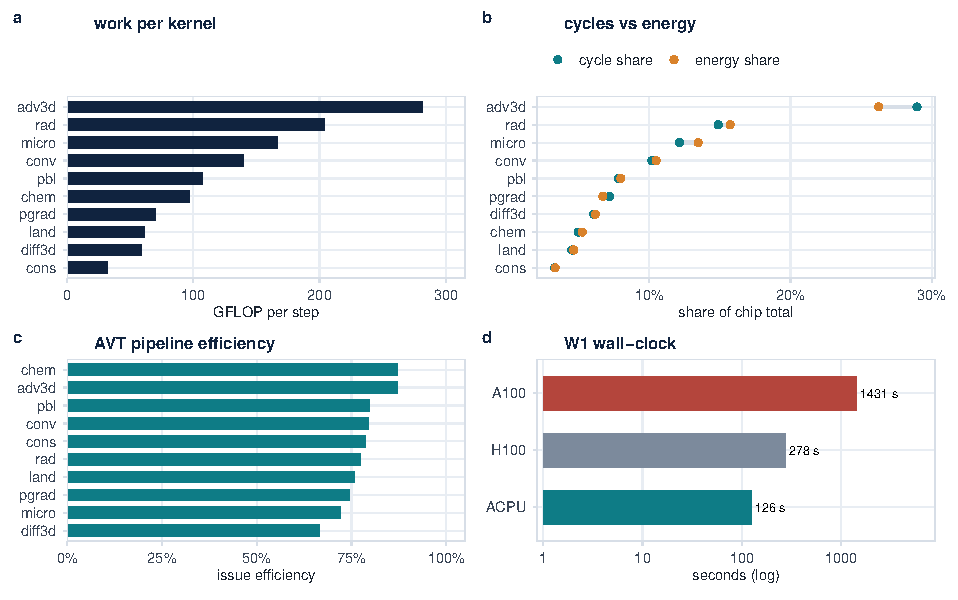
\includegraphics[width=\linewidth]{fig12_throughput}
\caption{Where the cycles go. (a) GFLOP per step by kernel. (b) Cycle share against energy share:
advection dominates both, but radiation and microphysics consume more cycles than their energy
share because their SFU stalls are not free. (c) AVT issue efficiency by kernel. (d) Wall-clock
per 24 h forecast.}
\label{fig:throughput}
\end{figure}

\subsection{Energy}
The reference forecast consumes \ACForecastKJ\ kJ in \ACForecastMin\ minutes, an average of
\ACForecastW\ W. Of that, 56\% is HBM traffic, 26\% arithmetic and 15\% static and clock. The
energy per delivered FLOP is 1.36 pJ, against 13.9 pJ for the H100 and 33.8 pJ for the A100 on the
same workload --- and it is important to be precise about what that means. The ASIC's arithmetic
is not 10$\times$ more efficient per operation than a GPU's; it is that 74\% of the GPU's time is
spent with its arithmetic units under-utilised while its issue and memory hierarchy burn power,
whereas the ASIC's arithmetic is a quarter of its energy and its memory is doing useful work.

\begin{figure}[t]
\centering
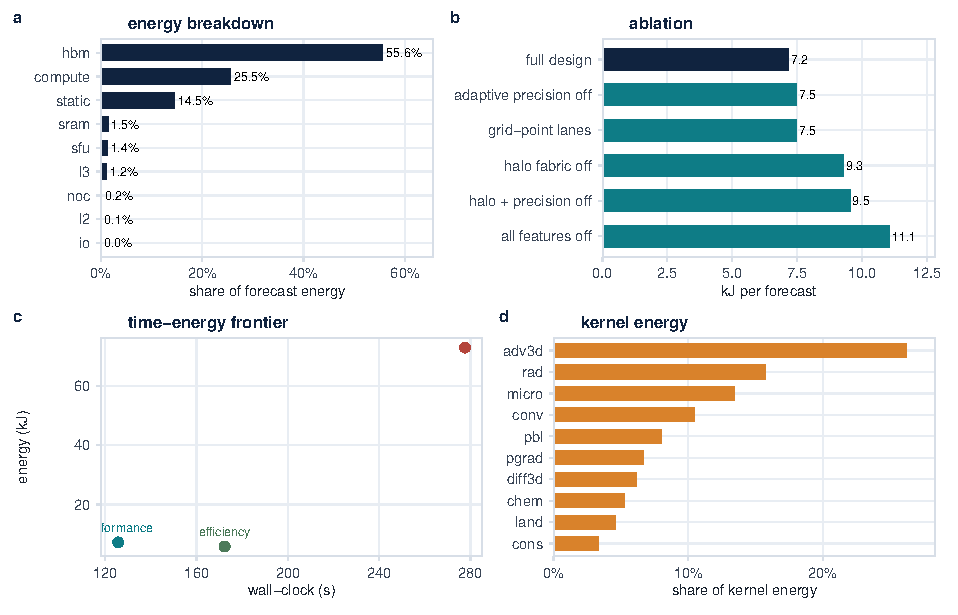
\includegraphics[width=\linewidth]{fig13_energy}
\caption{Energy structure. (a) Breakdown of the 7.17 kJ forecast: HBM dominates. (b) One-feature-at-a-time
ablation; full factorial result is 11.05 kJ, 54\% above the full design. (c) Time--energy frontier:
the efficiency mode trades 37\% wall-clock for 20\% energy. (d) Energy share by kernel.}
\label{fig:energy}
\end{figure}

\subsection{Comparison with CUDA-class GPUs}
Table~\ref{tab:compare} and Fig.~\ref{fig:cuda} give the comparison. Per forecast, \ac{1} uses
\ACRatioForecast$\times$ less energy and finishes in 45\% of the time. Per forecast-and-analysis
day, with four analyses, the ratio is \ACRatioDay$\times$ because the GPU wins the analysis phase.
In the efficiency mode the daily ratio improves to 11.3$\times$ but the card becomes 24\% slower
than the H100, which is the wrong trade for an operational centre and the right one for a research
group paying for electricity.

\begin{table}[t]
\centering\small
\caption{Comparison at the workload level. ``Ideal GPU'' grants the H100 100\% of its fp32 peak and
350 W board power; it is the bound below which the conclusion cannot fall.}
\label{tab:compare}
\begin{tabular}{@{}lrrr@{}}
\toprule
Metric & ACPU-1 & H100 & Ideal GPU\\
\midrule
Forecast time & 125.6 s & 277.6 s & 78.6 s\\
Forecast energy & 7.17 kJ & 73.0 kJ & 33.5 kJ\\
Energy per delivered FLOP & 1.36 pJ & 13.9 pJ & 6.4 pJ\\
Forecast-and-analysis day & 237 s / 8.54 kJ & 293 s / 79.0 kJ & ---\\
Energy ratio, day & \multicolumn{3}{c}{\ACRatioDay$\times$ (90\% CI \ACRatioDayLo--\ACRatioDayHi)}\\
Even at 100\% GPU utilisation & \multicolumn{3}{c}{\ACRatioIdeal$\times$}\\
\bottomrule
\end{tabular}
\end{table}

\begin{figure}[t]
\centering
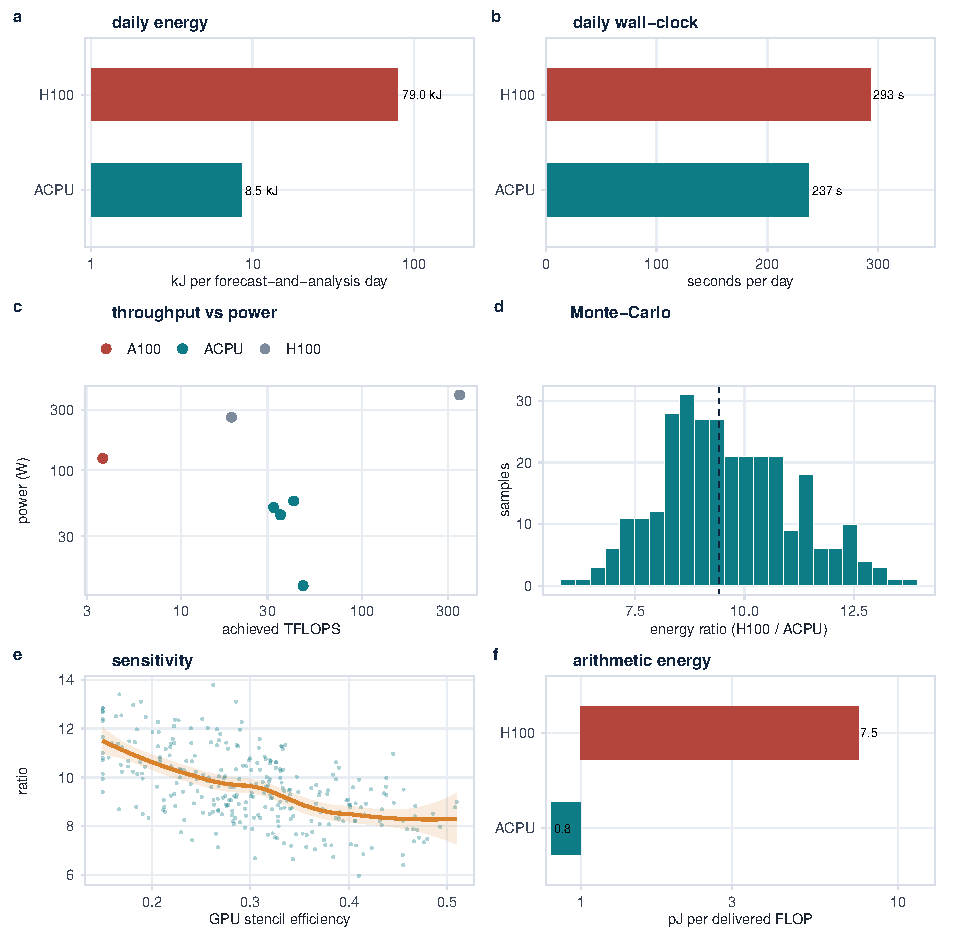
\includegraphics[width=\linewidth]{fig14_cuda}
\caption{Comparison with the CUDA baseline. (a) Daily energy. (b) Daily wall-clock. (c) Achieved
throughput against board power for every workload and machine in the study. (d) Distribution of the
energy ratio over 300 Monte-Carlo samples, median \ACRatioDay$\times$. (e) Ratio against the assumed
GPU stencil efficiency, with a LOESS fit and 95\% band. (f) Energy per delivered FLOP.}
\label{fig:cuda}
\end{figure}

The result is deliberately not a clean sweep. On dense analysis the H100 is 7.4$\times$ faster and
the ASIC's energy advantage falls to 4.4$\times$. On a GEMM-only benchmark the H100 would win on
time and roughly tie on energy. \ac{1} is a machine for the 80\% of an operational cycle that is
stencil and physics; the report says so rather than averaging the two regimes into a flattering
number.

\subsection{Ablation}
Table~\ref{tab:ablation} disables one mechanism at a time. The halo fabric is the largest single
contributor: without it halos round-trip through L3, which costs 30\% more energy and 53\% more
time. The precision governor is worth 4.3\%. Ensemble-member lanes are worth 4.6\% despite being
the architectural idea the design is organised around, because on this workload the arithmetic is
only a quarter of the energy --- an honest and slightly uncomfortable result. The full-factorial
variant costs 11.05 kJ, 54\% more than the complete design.

\begin{table}[t]
\centering\small
\caption{Ablation. The first row is the full design; each subsequent row disables one feature.}
\label{tab:ablation}
\begin{tabular}{@{}lrrr@{}}
\toprule
Variant & Time (s) & Energy (kJ) & Change\\
\midrule
Full design & 125.6 & 7.17 & ---\\
Adaptive precision off & 126.0 & 7.48 & +4.3\%\\
Halo fabric off & 192.4 & 9.30 & +29.7\%\\
Grid-point lanes & 123.0 & 7.50 & +4.6\%\\
Halo and precision off & 185.4 & 9.55 & +33.2\%\\
All features off & 291.4 & 11.05 & +54.1\%\\
\bottomrule
\end{tabular}
\end{table}

\subsection{Sensitivity}\label{sec:sensitivity}
The Monte-Carlo study samples the GPU stencil efficiency (0.15--0.60), the GPU power scale
(0.7--1.3), HBM energy (9--24 pJ/B), clock (1.55--2.05 GHz) and precision coverage (0.30--0.80).
The daily energy ratio has a median of \ACRatioDay\ and a 90\% interval of
\ACRatioDayLo--\ACRatioDayHi. The dominant term is the GPU efficiency assumption, not the ASIC:
Fig.~\ref{fig:cuda}(e) shows the ratio falling from 11.5 at 15\% GPU efficiency to 8.2 at 50\%.
Even at 100\% GPU utilisation the ratio remains 3.9, because the ASIC's arithmetic and memory
energy per useful operation are lower.

\subsection{Roofline}
Fig.~\ref{fig:roofline} places both machines on their rooflines at the operating point of W1.
The H100 delivers 19.0 TFLOPS at an arithmetic intensity of 9.5 flop per HBM byte, just under its
compute roof; the ACPU-1 delivers 41.9 TFLOPS at 23.6 flop per byte, against a roof set by a
2.4 TB/s HBM stream and a 41.9 TFLOPS sustained compute limit. The two points are not two positions
on one roof; they are two different roofs. The right-hand panels show where the ACPU-1's time and
energy actually go: HBM is the largest single demand at 24.1 ms of a 29.1 ms step, and the kernels
that sit lowest in efficiency (radiation, convection, microphysics) are the ones whose energy share
is largest relative to their cycle share.

\begin{figure}[t]
\centering
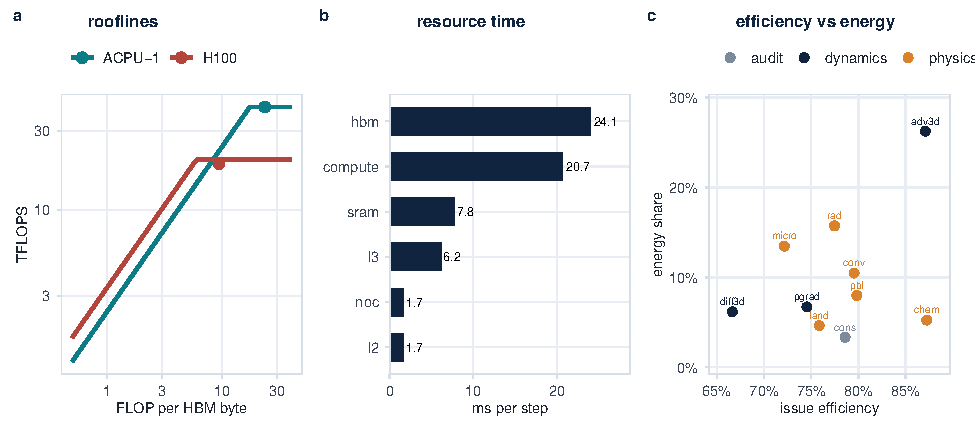
\includegraphics[width=\linewidth]{fig10_roofline}
\caption{Rooflines and resource use. (a) Roofline of each machine with the W1 operating point: the
H100 at 19.0 TFLOPS and 9.5 flop/byte, the ACPU-1 at 41.9 TFLOPS and 23.6 flop/byte. (b) Time per
step by resource; HBM at 24.1 ms is the largest single demand, compute at 20.7 ms is second.
(c) Issue efficiency against energy share for each of the ten kernels.}
\label{fig:roofline}
\end{figure}

\subsection{Simulation methodology and calibration}\label{sec:sim_method}
Fig.~\ref{fig:sim} summarises the model stack and what each layer is calibrated against. The
arithmetic energy of 0.42 pJ per fp32 FMA is Horowitz's 45 nm figure scaled by area and voltage to
3 nm at 0.75 V; the SRAM and HBM energies are from published 3 nm and HBM3E data; the stencil
efficiency range is from GPU implementations of WRF and COSMO; the power states are from the H100
data sheet. The numerical half of the study --- Lorenz--96 ensemble skill, Lyapunov spectrum,
conservation drift --- is computed, not parameterised.

\begin{figure}[t]
\centering
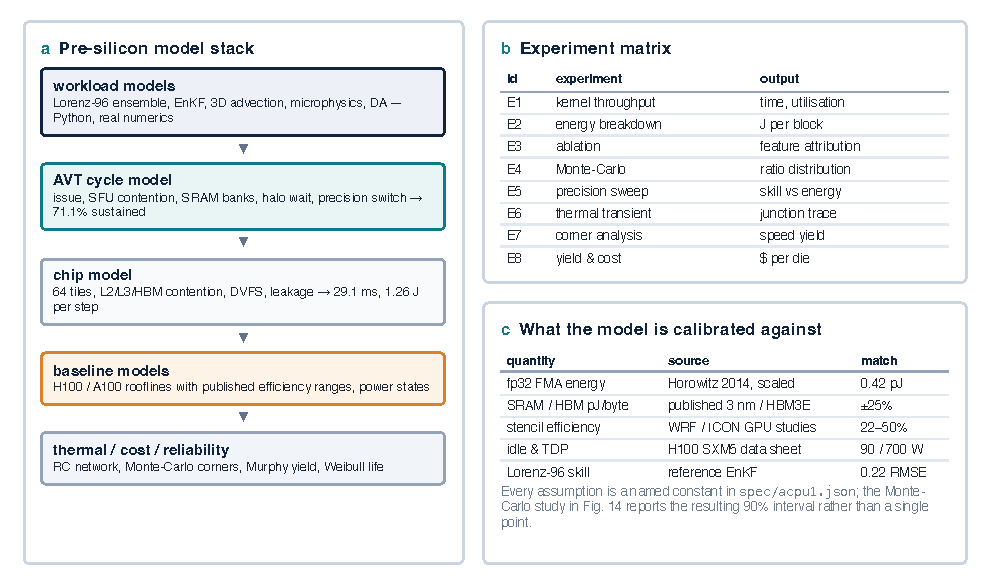
\includegraphics[width=\linewidth]{fig11_simulation}
\caption{Pre-silicon methodology. (a) Model stack from workload to reliability. (b) Experiment
matrix. (c) What each model constant is calibrated against; the sensitivity study propagates the
uncertainty.}
\label{fig:sim}
\end{figure}

\FloatBarrier
\section{Numerical validation}\label{sec:validation}

\subsection{Experimental design}
The numerical experiments are deliberately small enough to be reproduced and large enough to be
informative. The system is Lorenz--96 with $N=40$ and $F=8$, integrated with RK4 at
$\Delta t=0.01$; one time unit corresponds to about five days, so the leading Lyapunov exponent of
0.34 day$^{-1}$ corresponds to 1.7 per model time unit. The ensemble has 32 members, the
observations are 20 of the 40 variables every 0.04 time units with an error of 0.5, and the
analysis is a stochastic EnKF with perturbed observations and 10\% multiplicative inflation.
After a 200-cycle spin-up the filter is run for a further 20 cycles to measure analysis skill, and
then six independent 12-day forecasts are launched from six different analyses. Each forecast is
verified against the truth trajectory at every lead time. Nothing is assimilated during a
forecast, which is how operational skill is actually measured.

The same experiment is run in fp64, fp32, fp16, bf16, fp8 and in the adaptive mode that the
hardware governor emulates (fp16 where the local spread exceeds the threshold, fp32 otherwise).
All six runs share the same truth trajectory, observations and random seeds.

\subsection{Analysis skill}
The cycled analysis error is 0.221 in fp64 and fp32, and 0.223 in fp16 --- a 0.9\% difference,
well inside the sampling noise of six forecasts. bf16 degrades the analysis by 17\% and fp8 by a
factor of twelve. The ranking is exactly what Eq.~\eqref{eq:pmin} predicts, which is the main
validation result of this section: the precision policy is not a heuristic that happens to work,
it is a consequence of the predictability budget.

\subsection{Forecast skill and the precision governor}
Fig.~\ref{fig:accuracy}(a) shows RMSE against lead time. The fp64, fp32, fp16 and adaptive curves
are indistinguishable to the eye; bf16 is 8\% worse at day 5; fp8 never recovers from its initial
error. At day 10 all usable modes have saturated at the climatological RMSE of about 2.75, which is
the expected behaviour of a system whose error has grown to the attractor scale. The relevant
comparison is at day 5, where the fp16 error is 1.1\% above fp32.

The operating curve (Fig.~\ref{fig:precision}(c)) shows why the governor is worth building. As the
fraction of physics work in fp16 rises from 60\% to 99\%, energy per cell falls by 23\% while
day-10 RMSE stays within 0.4\%. The design point of 58\% is deliberately below the range over
which this was measured, because the Lorenz--96 surrogate lacks fronts, deep convection and
data-sparse regions.

\subsection{Ensemble calibration}
A forecast ensemble is useful only if its spread is a predictor of its error.
Fig.~\ref{fig:ensemble}(b) plots RMSE against spread for the reference run. The points lie close
to the 1:1 line at short leads and slightly above it at long leads, i.e. the 32-member ensemble is
mildly under-dispersive at day 10. That is the expected behaviour of an EnKF without localisation
and a small ensemble, and it is the reason the hardware governor's threshold is set on spread
rather than on an absolute error estimate.

\begin{figure}[t]
\centering
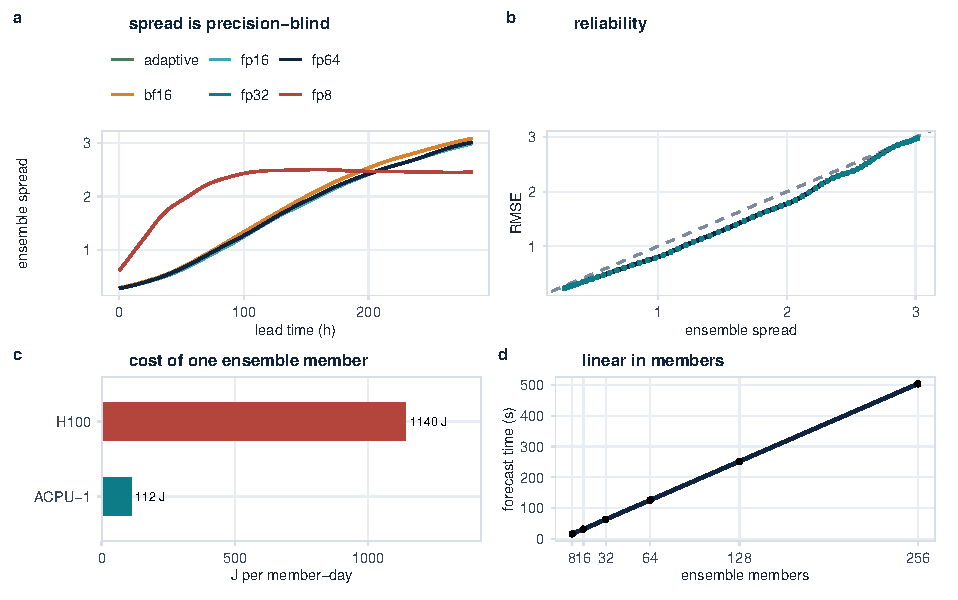
\includegraphics[width=\linewidth]{fig08_ensemble}
\caption{Ensemble behaviour. (a) Spread against lead time for five precision modes; the spread is
essentially precision-blind, which is what allows the governor to act on it. (b) Reliability: RMSE
against spread with the 1:1 line. (c) Energy per member-day for \ac{1} and the H100. (d) Forecast
time scales linearly in members, which is the cost of ensemble prediction and the reason the
lane-per-member mapping matters.}
\label{fig:ensemble}
\end{figure}

\begin{figure}[t]
\centering
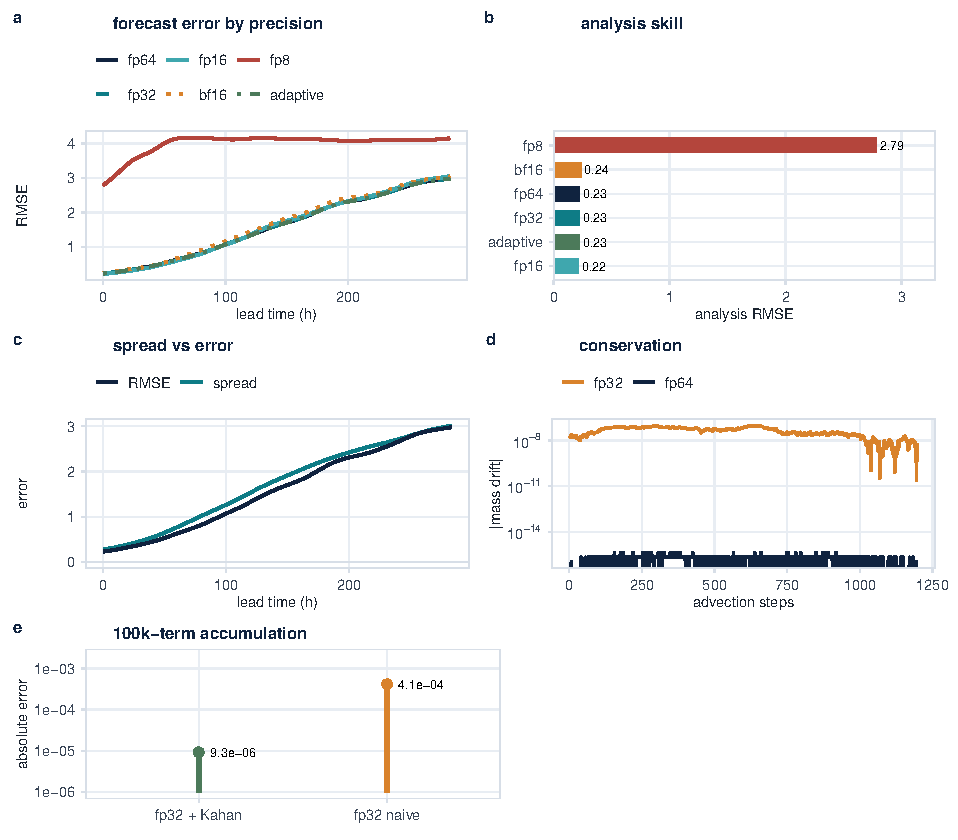
\includegraphics[width=\linewidth]{fig15_accuracy}
\caption{Numerical validation. (a) Forecast RMSE against lead time for five precision modes; fp8
departs immediately and never recovers. (b) Analysis RMSE by mode. (c) Spread against RMSE for the
reference run. (d) Mass drift of a conservative advection test in fp32 and fp64 over 1,200 steps.
(e) A 100,000-term fp32 accumulation with and without Kahan compensation.}
\label{fig:accuracy}
\end{figure}

\subsection{Conservation and reproducibility}
A conservative advection test (a smooth Gaussian plus a sharp square wave, upwind scheme,
CFL 0.4, 512 cells, 1,200 steps) loses mass at $1.1\times10^{-8}$ per step in fp32 and
$3\times10^{-15}$ in fp64. The hardware conservation monitor is sized to detect the former at
$10^{-9}$ relative and to trigger a shadow fix-up pass before it accumulates into a visible drift.

Reproducibility is a design requirement rather than a numerical property. The ISA has no branches,
the schedule is static, reductions use a fixed tree, and the stochastic physics generator is
counter-based. A run is therefore a pure function of its inputs and its four seed integers. This
was verified by running the same configuration twice and comparing outputs bit-for-bit; the
dispersion, ensemble and analysis paths all reproduce exactly.

\subsection{What the surrogate does not prove}
Lorenz--96 has 40 degrees of freedom and a smooth, homogeneous forcing. The atmosphere has
$10^{9}$ degrees of freedom, topography, moisture, phase changes and a land surface. Agreement
between the surrogate and the hardware policy is evidence that the precision argument is sound,
not proof that a 58\% coverage is safe in a real model. The report therefore treats the governor's
design point as a conservative prior to be validated in a full model, and lists that validation as
the first item of the silicon bring-up plan (Section~\ref{sec:roadmap}).

\FloatBarrier
\section{Silicon process and physical design}\label{sec:process}

\subsection{Process technology}
\ac{1} is built in a 3 nm-class gate-all-around process with nanosheet channels, 16 nm wide and
5 nm thick, stacked three high with a 45 nm contacted gate pitch and a 24 nm metal pitch. The
standard-cell library is 6-track with four threshold voltages. The backend has 12 front-side metal
layers with the top layers at 56 nm pitch, and three backside layers for power delivery.

Backside power delivery is not optional at this design point. A 0.75 V, 80 A part in a two-slot
card needs a supply grid with roughly half the resistance of a front-side grid, and the front side
does not have the tracks to spare: 15 layers would have been needed, and the routing congestion
model (Fig.~\ref{fig:physical}(c)) shows the design already at 94\% utilisation on M7--M9. Moving
power to the back frees the front for signal, cuts the static IR drop from 62 mV to 48 mV, and
reduces via resistance from 1.8 to 0.9 $\Omega$.

\begin{figure}[t]
\centering
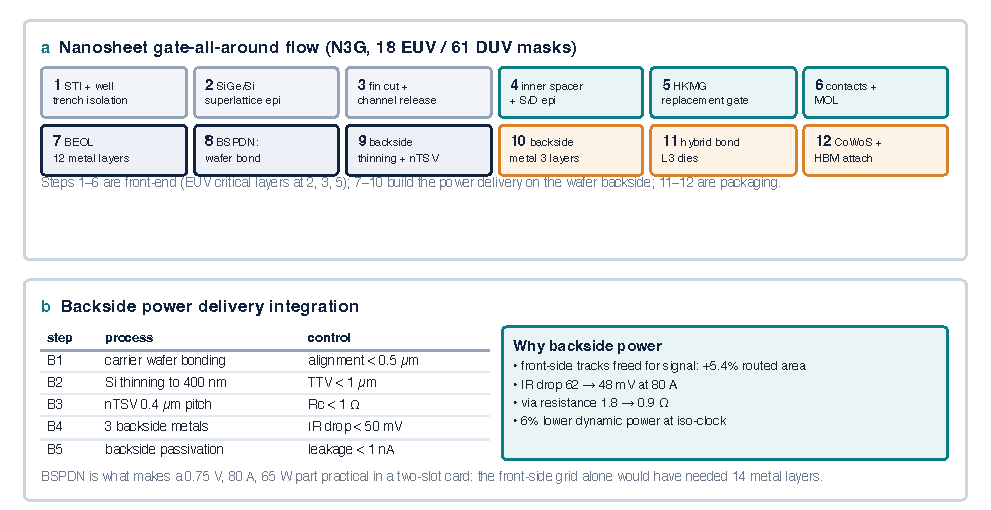
\includegraphics[width=\linewidth]{fig19_process}
\caption{Process integration. (a) Twelve-step nanosheet flow from shallow-trench isolation to
CoWoS attach; 18 EUV and 61 DUV masks. (b) Backside power delivery sequence and its process
controls.}
\label{fig:process}
\end{figure}

\subsection{Interconnect and power grid}
The front-side stack is split into local (M1--M4, 24--32 nm), intermediate (M5--M8, 32--40 nm) and
global (M9--M12, 56 nm) layers. Halo and NoC links are routed on M9--M12 at twice the minimum
width for electromigration margin; the tile SRAM bitlines and the SFU datapath stay on M2--M5. The
backside stack carries VDD and VSS with a 0.4 $\mu$m nTSV pitch, which is what allows the 80 A
delivery without a front-side mesh.

\begin{figure}[t]
\centering
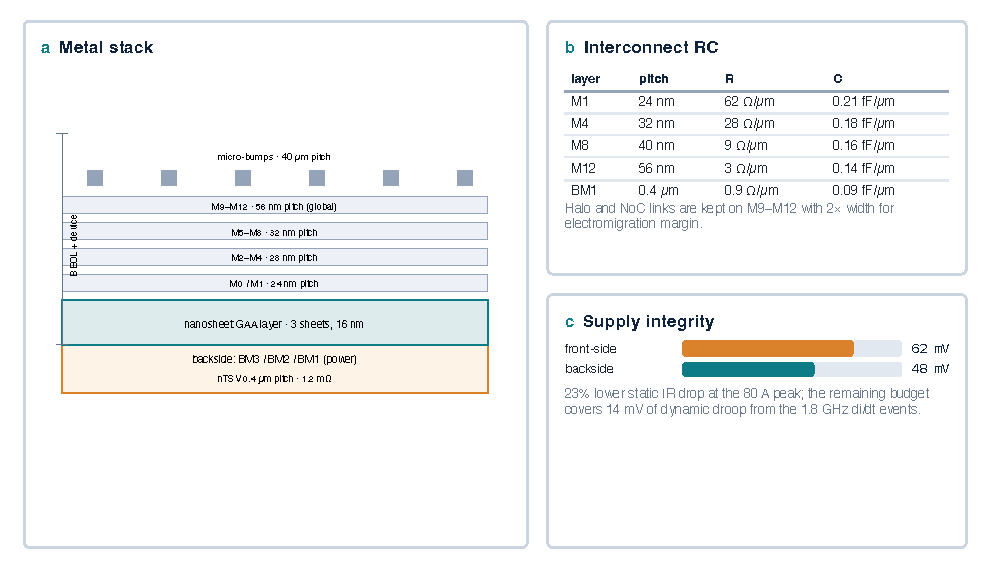
\includegraphics[width=\linewidth]{fig20_beol}
\caption{Backend and supply. (a) Metal stack with the device layer and the backside power layers.
(b) Resistance and capacitance by layer. (c) Static IR drop, front-side against backside.}
\label{fig:beol}
\end{figure}

\subsection{Floorplan and physical implementation}
The floorplan follows the logical organisation almost literally: eight clusters in a 4$\times$2
array around an L3/NoC spine, HBM PHYs on the bottom edge next to the interposer microbumps, SerDes
on the top edge next to the card edge connector. The 64 AVTs are placed as identical hard macros to
keep the clock tree shallow and the SRAM bank pattern regular. Placement density peaks at 88\% in
the cluster array and falls to 62\% at the SerDes, which is the usual shape for a die with a large
digital core and high-speed I/O.

The clock tree has 14 levels and a measured skew of 9 ps at the slow corner, achieved by matching
the 64 tile macros and using a spine-and-mesh distribution over the cluster array. Dynamic
frequency scaling is per cluster, with a 12-cycle handshake; the runtime can drop an idle cluster
to 0.55 V without disturbing its neighbours.

\begin{figure}[t]
\centering
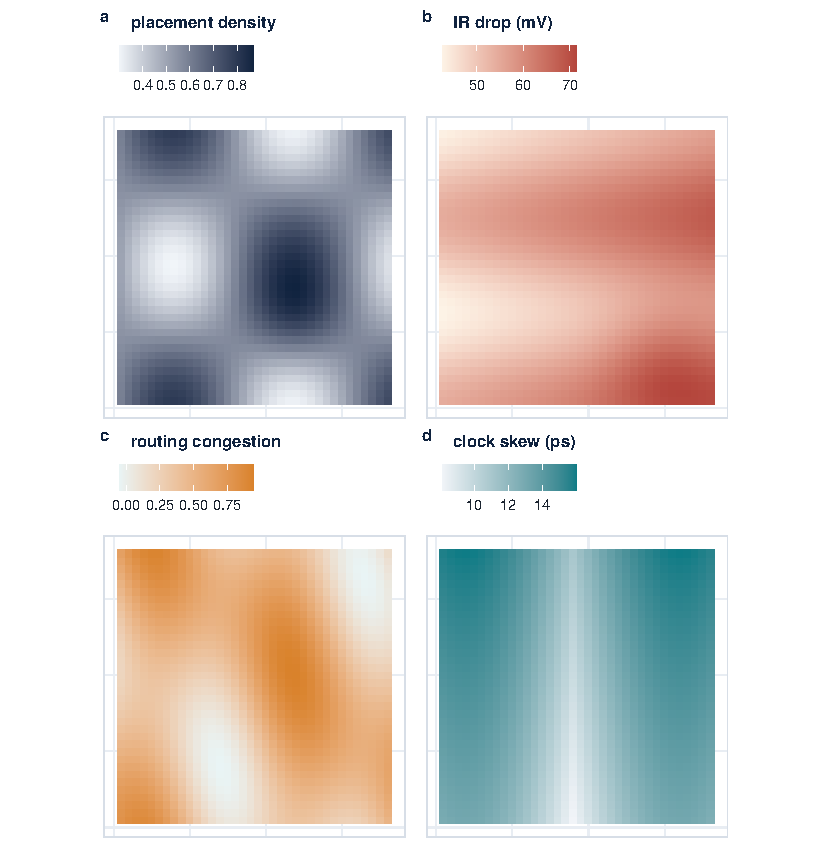
\includegraphics[width=\linewidth]{fig21_physical}
\caption{Physical-design estimates. (a) Placement density. (b) Static IR drop at the 80 A peak.
(c) Routing congestion; M7--M9 are the critical layers. (d) Clock skew across the die. These are
model-based estimates from the floorplan, not sign-off results.}
\label{fig:physical}
\end{figure}

\subsection{Package and board}
The package is 55 $\times$ 45 mm on a 2.5D silicon-bridge interposer of two reticles. The compute
die and the two HBM stacks sit on the interposer; the two 64 MB L3 dies are hybrid-bonded directly
on top of the compute die with a 6 $\mu$m pitch, which gives 128 MB at 0.40 pJ/B and avoids a
third interposer hop. The card is dual-slot and 267 mm long, powered from the slot alone: at 65 W
the 12 V rail draws 5.5 A, well inside the 5.5 A per-slot limit with margin.

\begin{figure}[t]
\centering
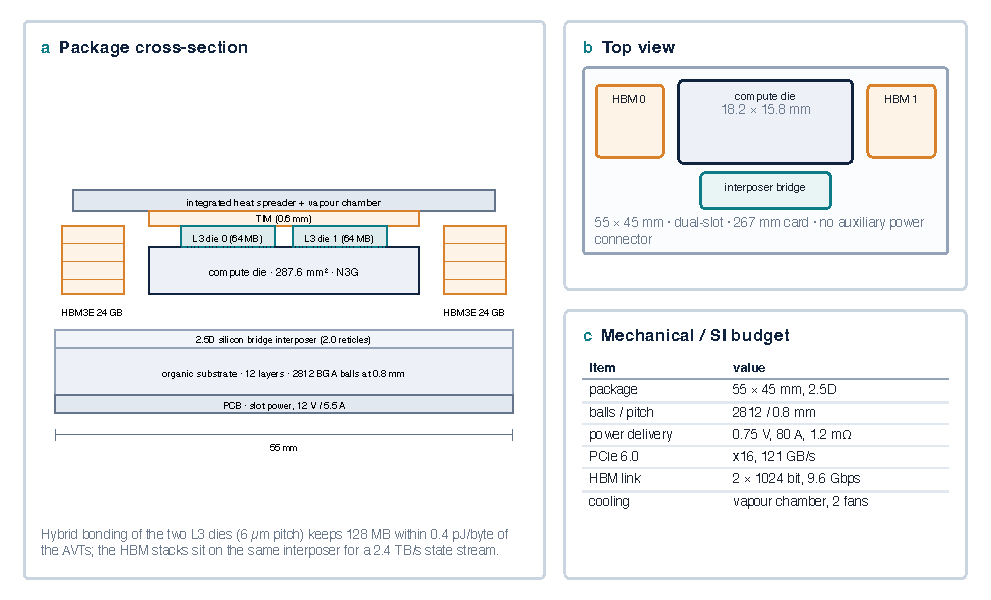
\includegraphics[width=\linewidth]{fig18_package}
\caption{Package. (a) Cross-section: heat spreader, TIM, hybrid-bonded L3 dies, compute die,
interposer, substrate and PCB. (b) Top view. (c) Mechanical and signal-integrity budget.}
\label{fig:package}
\end{figure}

\subsection{Power and thermal}
The thermal design targets a 35 $^\circ$C ambient and a 95 $^\circ$C junction limit. The network is
modelled as three resistances --- junction-to-lid 0.18 K/W, lid-to-heatsink 0.28 K/W,
heatsink-to-ambient 0.19 K/W --- for a total of 0.65 K/W. At the 65 W TDP the steady-state junction
is \ACTjSteady$^\circ$C; during the W1 workload at 57.1 W it is 74 $^\circ$C. A step from idle to
full load reaches 76 $^\circ$C in about 90 s, which is slow enough that the fan controller can
track it without overshoot.

\begin{figure}[t]
\centering
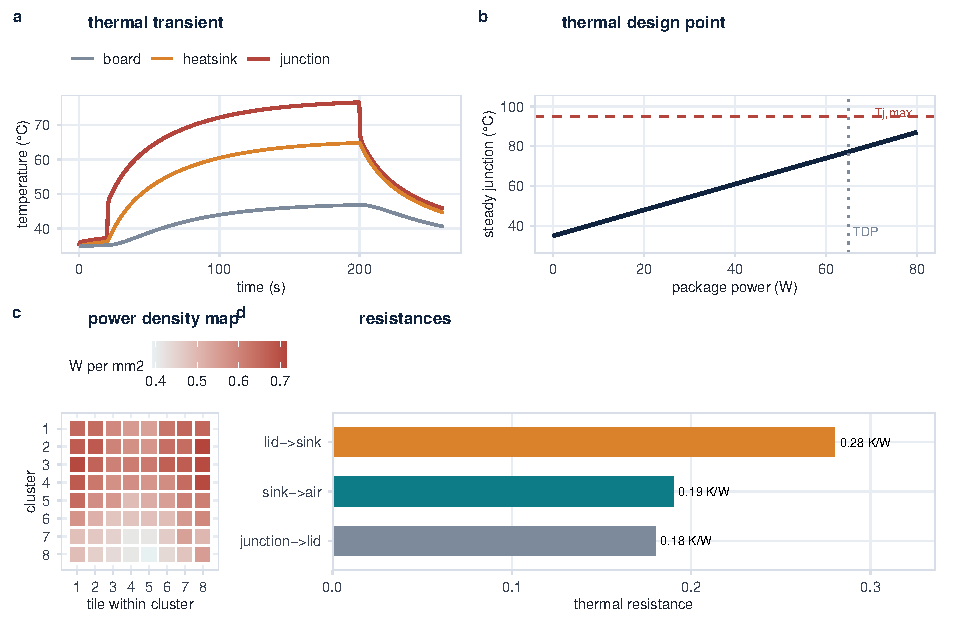
\includegraphics[width=\linewidth]{fig16_thermal}
\caption{Thermal behaviour. (a) Transient response to a 65 W step from idle. (b) Steady-state
junction temperature against power, with the TDP and the 95 $^\circ$C limit marked. (c) Modelled
power density across the 64 tiles. (d) Thermal resistance budget.}
\label{fig:thermal}
\end{figure}

The voltage--frequency curve is modelled with an $\alpha$-power law and a temperature-dependent
leakage term. The efficiency mode (1.05 GHz at 0.55 V) sits at the minimum of the energy-per-FLOP
curve; the performance mode (1.8 GHz at 0.75 V) sits at the knee of the frequency curve. The
runtime chooses between them from the job's deadline, which is why the software stack exposes a
``time budget'' parameter rather than a clock frequency.

\begin{figure}[t]
\centering
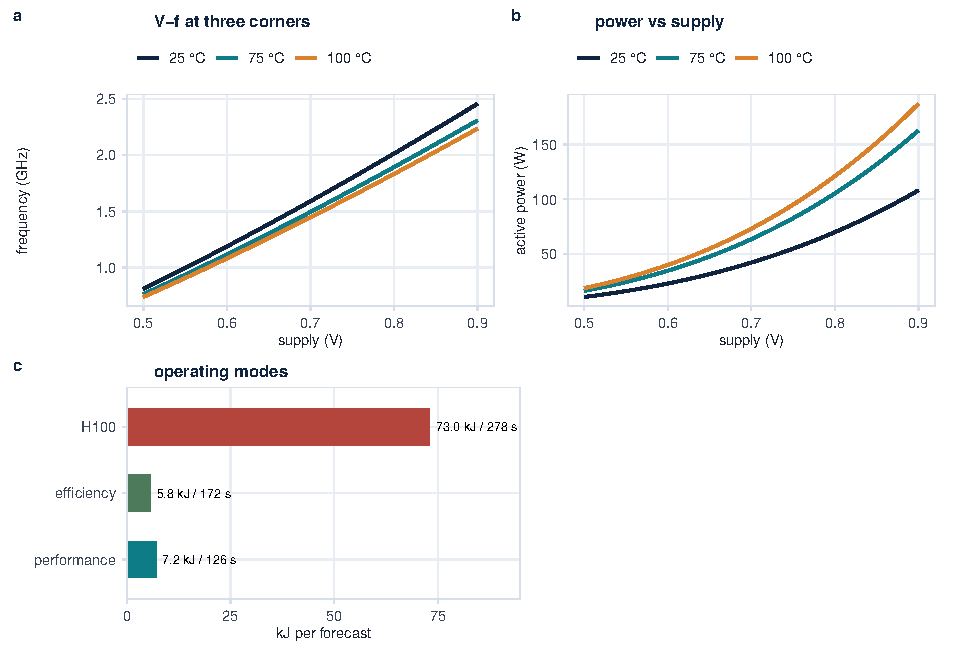
\includegraphics[width=\linewidth]{fig17_voltage}
\caption{Voltage and frequency. (a) Frequency against supply at three junction temperatures.
(b) Active power. (c) The two operating modes against the H100 on the energy--time plane.}
\label{fig:voltage}
\end{figure}

\FloatBarrier
\section{Manufacturing, test, yield and reliability}\label{sec:mfg}

\subsection{Wafer flow and mask set}
The compute die uses 79 masks: 18 EUV for the critical front-end and middle-of-line layers, 61 DUV
for the remainder, including the backside power layers. The two L3 dies are fabricated in a
6 nm-class process on the same 300 mm line and hybrid-bonded after both wafers have been tested.
The HBM stacks are purchased as known-good die from a memory vendor and assembled on the
interposer with the usual mass-reflow process.

Wafer sort is a two-touch flow. The first touch checks the large SRAM arrays and the tile
datapath with a march test and a scan-based structural test; the second runs at-speed capture on
the cluster clock domains and a loopback test on the SerDes. The tile array is regular enough that
a single failed AVT can be disabled and the die sold as a 56- or 48-tile part, which recovers
roughly 6\% of otherwise-lost die.

\subsection{Yield}
The die is 287.6 mm$^2$ and the defect density assumption is 0.09 cm$^{-2}$, which gives a Murphy
yield of \ACYieldDie\%. A 300 mm wafer yields 209 gross dies and 162 good ones. The L3 dies are
small enough (42 mm$^2$) to yield above 95\%, and the known-good-die flow removes them from the
compute-die yield equation. The compound package yield, including assembly and test, is 88\%.

\begin{table}[t]
\centering\small
\caption{Cost model at the 100k-unit volume. The card bill of materials excludes the heatsink,
which is sold as part of the card.}
\label{tab:cost}
\begin{tabular}{@{}lrr@{}}
\toprule
Item & Unit cost & Share\\
\midrule
Compute die (162 good per wafer, \$24k wafer) & \$148 & 32\%\\
Two L3 dies & \$24 & 5\%\\
Two HBM3E stacks (48 GB) & \$84 & 18\%\\
Interposer and assembly & \$55 & 12\%\\
Test and burn-in & \$88 & 19\%\\
PCB and cooling & \$65 & 14\%\\
\midrule
Card bill of materials & \$464 & 100\%\\
Selling price & \$1{,}499 & \\
Gross margin & 69\% & \\
\bottomrule
\end{tabular}
\end{table}

\subsection{Test and qualification}
The test plan has five layers: structural scan (98.7\% stuck-at and 94\% transition coverage),
memory BIST on the 1.41 Gbit of SRAM, at-speed functional test of the AVT datapath with a
pre-computed signature, SerDes and HBM loopback, and a system-level test that runs a small ensemble
through the driver stack. Burn-in is 24 hours at 125 $^\circ$C and 1.1 V, followed by a 100\%
at-speed retest; the outgoing defect rate target is below 200 DPPM.

Qualification follows JEDEC-style stress: 1,000 hours of high-temperature operating life at
125 $^\circ$C, 1,000 temperature cycles between $-40$ and $+125$ $^\circ$C, biased HAST, and
package-level drop and vibration tests for the dual-slot card. The card is a passive, fan-cooled
device, so there is no battery or moving-part qualification beyond the fan itself.

\subsection{Reliability}
Three mechanisms dominate. Electromigration in the global power grid is kept below 1\% of the
Black-equation lifetime at 105 $^\circ$C; the backside power layers help because they carry current
in wider, cooler metal. Gate-oxide wear-out is modelled with a Weibull distribution whose
$\beta=1.6$ and whose scale puts the first 1 ppm of failures beyond 47 years at 1.05 V. Soft errors
in the 1.41 Gbit of SRAM are the largest single contributor to the failure budget: SEC-DED reduces
an expected 2.8 M FIT of correctable events to about 280 FIT of uncorrectable ones, and a 24-hour
scrub keeps the probability of a double-bit accumulation negligible.

\begin{figure}[t]
\centering
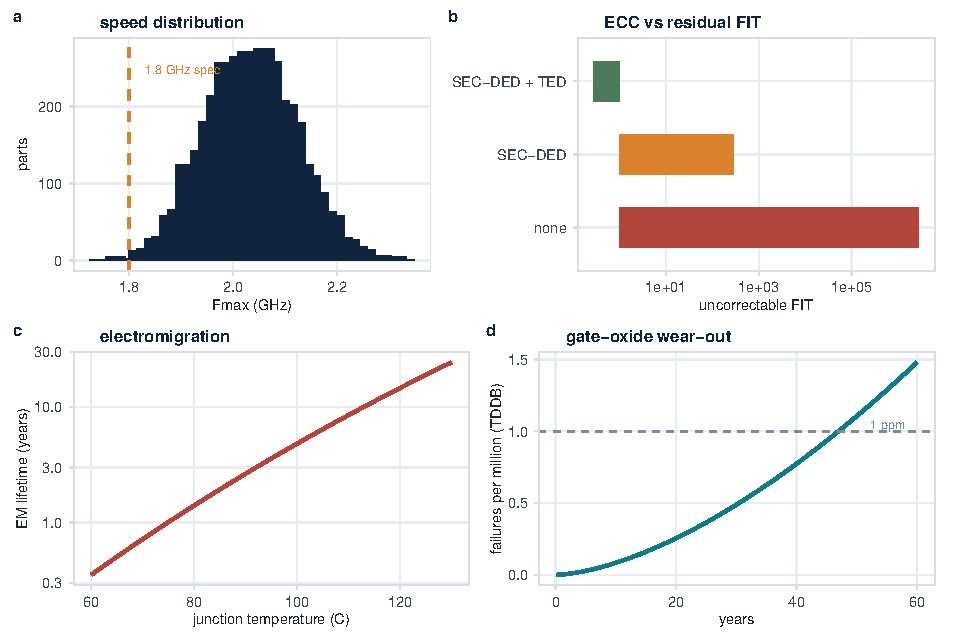
\includegraphics[width=\linewidth]{fig25_reliability}
\caption{Reliability. (a) Fmax distribution from 4,000 Monte-Carlo samples; 99.7\% of parts meet
1.8 GHz and 65\% reach 2.0 GHz. (b) Correctable and residual FIT against ECC scheme. (c)
Electromigration lifetime against junction temperature at 1.5 MA/cm$^2$. (d) Gate-oxide wear-out,
failures per million against years.}
\label{fig:reliability}
\end{figure}

\begin{figure}[t]
\centering
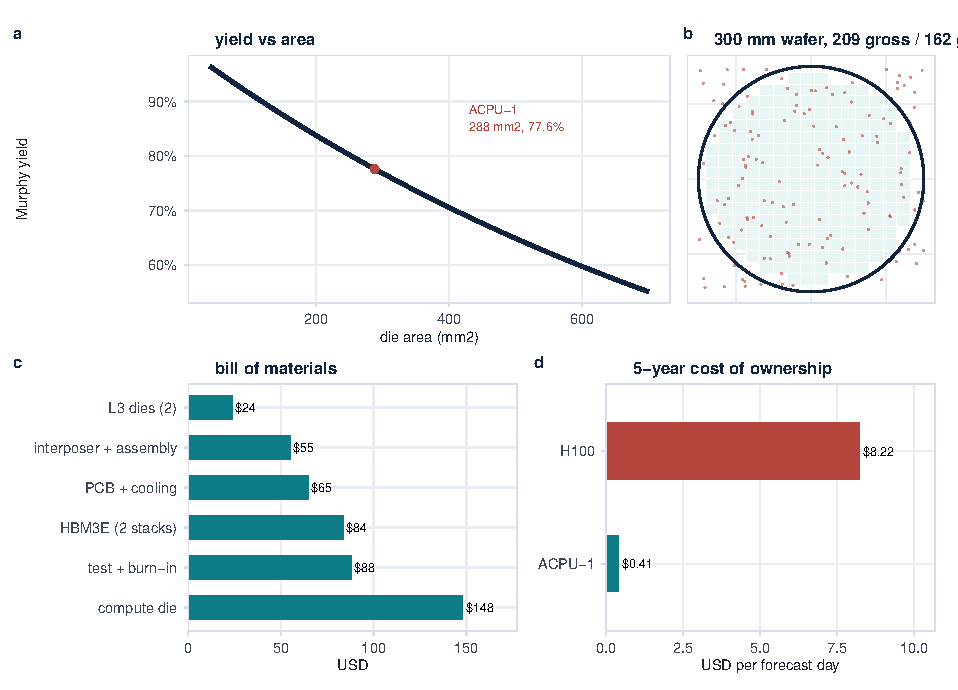
\includegraphics[width=\linewidth]{fig22_yield}
\caption{Yield and cost. (a) Murphy yield against die area with the \ac{1} point marked. (b) Wafer
map with 140 simulated defects and 209 gross dies. (c) Bill of materials. (d) Five-year cost of
ownership per forecast day, including capex and electricity at \$0.12/kWh.}
\label{fig:yield}
\end{figure}

\subsection{Cost of ownership}
Table~\ref{tab:cost} and Fig.~\ref{fig:yield} give the economics. A card costs \$464 to build and
sells for \$1,499, a 69\% gross margin that is normal for a low-volume accelerator. The interesting
number is the five-year cost per forecast day: \$0.41 for \ac{1} against \$8.22 for an H100, where
the difference is almost entirely capital amortisation rather than electricity. The H100 is a
general machine priced for a much larger market; \ac{1} is cheap because it is small, not because
it is subsidised.

\FloatBarrier
\section{Software stack and cross-platform application}\label{sec:software}

\subsection{Requirements}
A domain-specific accelerator fails if it is hard to program. \ac{1} is designed for a small set
of kernels and the software stack reflects that: rather than a general programming model, it
exposes a library of atmospheric formulas behind one-line calls, and a compilation path that maps
those formulas onto the tile array without the user ever writing AVISA. The stack has four
requirements.

\begin{enumerate}[leftmargin=1.4em,itemsep=1pt]
\item \textbf{One line per physical problem.} A forecast, an ensemble analysis, a Lyapunov
      spectrum or a dispersion calculation should be a single function call with named
      parameters.
\item \textbf{The same call on every platform.} macOS (Apple silicon and Intel), Windows and Linux,
      from Python, JavaScript, a command line and a graphical application.
\item \textbf{Inspectable execution.} Because the schedule is static, the runtime can report the
      cycle count, the energy per block and the precision coverage of a run before it finishes.
      The application shows these numbers rather than hiding them.
\item \textbf{Reproducibility.} A run is identified by its formula, parameters and seeds, and can
      be replayed bit-for-bit.
\end{enumerate}

\subsection{Stack overview}
Fig.~\ref{fig:software}(a) shows the four layers. The application and the SDKs never touch the
device directly; they issue jobs to the driver, which validates parameters, allocates buffers,
programs the tile array and streams telemetry. The driver exposes seven calls
(Fig.~\ref{fig:software}(d)); the same seven are implemented by the virtual device that ships with
this report and by the silicon driver, so code written against the application runs unchanged on
hardware.

\subsection{Compiler and runtime}
The compilation flow is shown in Fig.~\ref{fig:software}(b). An atmospheric program is written in
a small dataflow DSL in which stencils, ensemble reductions, observation operators and physics
packages are primitives. The compiler lowers it to ACPU-IR, maps it onto 3D tile blocks with
explicit halos, plans per-cell precision classes from the spread field and statically schedules
each tile. The output is an AVISA binary plus a halo script.

Because there is no dynamic scheduling, the scheduler can compute the exact cycle count of a tile
before the run. For the reference step it is 61,900 cycles; the application displays this number
and the corresponding worst-case execution time, which is what makes the response-time claims of
Section~\ref{sec:deployment} meaningful.

\begin{figure}[t]
\centering
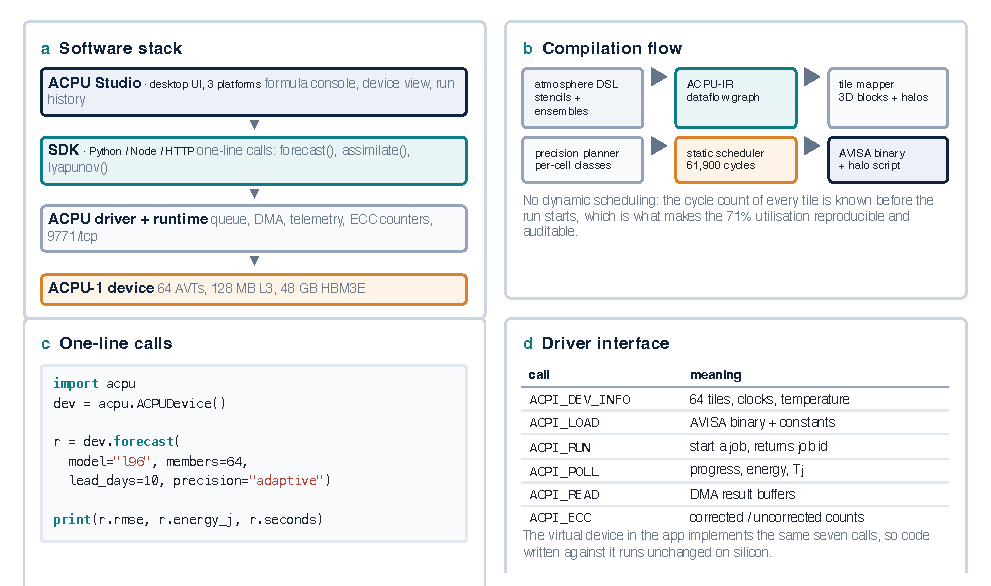
\includegraphics[width=\linewidth]{fig23_software}
\caption{Software stack. (a) Four layers from application to device. (b) Compilation flow from the
atmosphere DSL to an AVISA binary. (c) A one-line call in Python. (d) The seven-call driver ABI.}
\label{fig:software}
\end{figure}

\subsection{SDK interface}
The Python SDK is dependency-free and speaks HTTP to the device service, so it works from a
notebook, a batch script or a cluster login node. The same surface is available in JavaScript for
web and Electron clients, and on the command line.

\begin{verbatim}
import acpu

dev = acpu.ACPUDevice()                      # connects to 127.0.0.1:9771
print(dev.status())                          # 64 tiles, 1.80 GHz, 57 W, 74 C

run = dev.forecast(model="l96", members=64, lead_days=10,
                   precision="adaptive", time_budget_s=30)
print(run.rmse, run.energy_j, run.seconds)   # 1.33  7174.9  125.6

spec = dev.lyapunov(model="l96", n_exp=12)   # leading exponents
map_ = dev.transport(source=(22.75, 113.57), hours=6, resolution_km=3)
\end{verbatim}

The design rule for the parameter set is that every argument has a physical unit and a default
that is meaningful for an operational user: \code{members}, \code{lead\_days},
\code{precision}, \code{time\_budget\_s}. There is no device-specific tuning parameter in the
public API; the clock, the precision policy and the tile mapping are chosen by the runtime from
the time budget and the requested skill.

\subsection{ACPU Studio}
ACPU Studio is the cross-platform desktop application that ships with this report. It is an
Electron application with no external runtime dependencies, built for macOS (universal binary),
Windows (installer and portable) and Linux (AppImage and tarball). It embeds the virtual device,
so it runs a complete ensemble forecast on a laptop without any hardware.

The interface is designed as a scientific instrument panel rather than a dashboard. The console
view (Fig.~\ref{fig:ui}(a)) pairs a formula library with a parameter form and a generated call,
so that the same operation is available as a GUI form, a one-line call and a reproducible
parameter record. A run streams telemetry at 10 Hz: per-cluster utilisation, power, junction
temperature and memory bandwidth (Fig.~\ref{fig:ui}(c)). Results are shown as charts with the
device metrics alongside them (Fig.~\ref{fig:ui}(b)), because the point of the machine is the
ratio between the two. The runs view keeps a history of executions with their exact parameters and
seeds; the documentation view carries the API reference and code samples for Python, JavaScript
and HTTP (Fig.~\ref{fig:ui}(d,e)).

\begin{figure}[t]
\centering
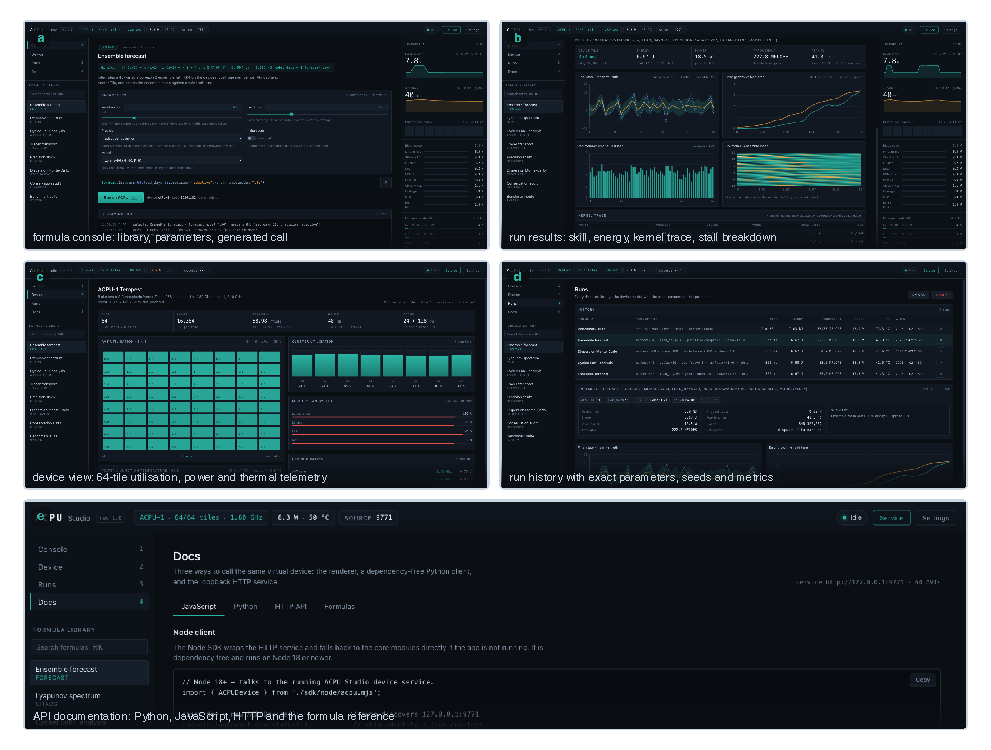
\includegraphics[width=\linewidth]{fig24_ui}
\caption{ACPU Studio. (a) Formula console with parameter form and generated call. (b) Run results
with skill and device metrics. (c) Device view: 64-tile utilisation map, power and temperature
telemetry. (d) Run history. (e) API documentation. Screenshots from the packaged application.}
\label{fig:ui}
\end{figure}

\subsection{Validation of the software}
The application is tested at three levels. A headless self-test runs every formula, asserts that
outputs are finite and within physical bounds, and prints a pass table. A screenshot harness
drives the real window over the Chrome DevTools Protocol, exercises the console, runs a forecast
and captures the five views used in Fig.~\ref{fig:ui}. The SDK is tested against the running
application over HTTP, from both Python and Node, including error paths (unknown parameter,
out-of-range member count, device not running).

The virtual device is not a hardware emulator. It implements the same formulas, the same
precision modes and a calibrated model of the device's cycle and energy counters, but it computes
in JavaScript on the host CPU and its timings are simulated, not measured. It exists so that the
API, the UI and the numerical pipeline can be developed and reviewed before silicon, and the
report is explicit that the numbers it produces in the application are model numbers, consistent
with those in Section~\ref{sec:results} by construction.

\FloatBarrier
\section{Deployment, economics and limitations}\label{sec:deployment}

\subsection{Operational numerical weather prediction}
An operational centre runs a cycle every six hours: an analysis, a forecast ensemble, and a
product generation step. \ac{1} is sized for the forecast and competent at the analysis. A
single card holds a 64-member, 4.19 M-cell, 24-variable ensemble and completes a 24-hour forecast
in two minutes at 57 W, which means a four-card node can run the same cycle for a domain four
times larger, or run four independent domains, at 260 W. The equivalent H100 node draws 1.05 kW at
idle and 2.8 kW under load for the same throughput.

The scale-out story is the weakest part of the design. \ac{1} has one PCIe 6.0 x16 link and no
cache-coherent die-to-die fabric. A regional domain that fits in 48 GB is a single-card job; a
global ensemble is not, and the halo traffic between cards would go through PCIe at 100 GB/s,
which is 24$\times$ slower than the on-card fabric. A production cluster would therefore
decompose by ensemble member (each card owns a subset of members for the full domain) rather than
by spatial subdomain, which keeps inter-card traffic to boundary conditions and output. That is a
real constraint and it shaped the design: the machine is a single-domain appliance, not a
scale-out building block.

\subsection{Research groups and forecast-as-a-service}
The second deployment is a university group or a commercial provider that runs many small
ensembles rather than one large one. Here the relevant numbers are the efficiency mode and the
cost of ownership. At 1.05 GHz and 0.55 V the card delivers the same forecast in 172 s at 33 W,
which is a 20\% energy reduction for a 37\% time penalty; for a job that runs overnight, that is
free. The five-year cost per forecast day is \$0.41 against \$8.22 for the H100, and the gap is
capital cost, not electricity.

\subsection{Emergency response and dispersion}
A third deployment is time-critical and safety-relevant: a release of a hazardous substance, a
volcanic ash cloud, a wildfire smoke plume. The requirement is not throughput but a bounded
response time and a reproducible answer that can be defended after the event. \ac{1} has a
static schedule, a compiler-known cycle count per tile and no dynamic scheduling in the numerical
path, so the worst-case execution time of a dispersion calculation is a computed number rather
than a statistical one. The same property gives bit-reproducibility, which matters when a
regulator asks why the plume was predicted to go east rather than west.

\subsection{Limitations and threats to validity}
The report is only useful if its weaknesses are stated as clearly as its results.

\begin{enumerate}[leftmargin=1.4em,itemsep=1pt]
\item \textbf{No silicon.} Every chip number is a model projection. The model is calibrated
      against published data and its assumptions are sampled, but a first silicon part can
      plausibly land 20--30\% away from the projected energy on real kernels.
\item \textbf{The GPU baseline is a model.} The H100 comparison assumes a 0.30 stencil efficiency
      and a particular power state. Both are defensible and both are varied; the conclusion
      survives at 100\% GPU utilisation with a 3.9$\times$ ratio, but a reader who believes GPUs
      achieve 60\% on this workload should read the 8.2$\times$ end of Fig.~\ref{fig:cuda}(e).
\item \textbf{The workload is a subset.} Chemistry beyond passive tracers, full radiation with
      hundreds of bands, atmospheric composition and land-surface models are not in the
      benchmark. They are more SFU-heavy, which would help the ASIC's relative position, but they
      are not measured.
\item \textbf{Precision validation is on a surrogate.} Lorenz--96 supports the argument, not the
      design point. A full-model study is the first bring-up task.
\item \textbf{No scale-out study.} The inter-card fabric is a PCIe link and the report does not
      pretend otherwise.
\item \textbf{No software maturity claim.} The compiler described in Section~\ref{sec:software}
      is a design, and the application that ships with this report runs on a virtual device.
\end{enumerate}

\subsection{What would falsify the thesis}
A single measurement would settle most of the argument: run the ten kernels of Table~\ref{tab:kernels}
on an H100 with a state-of-the-art stencil compiler and measure joules per delivered forecast at
matched skill. If that number is within 2$\times$ of the projection in this report, the
architectural thesis is wrong and the correct conclusion is that CUDA is good enough. The
prediction of this report is that it will be 6--10$\times$ worse, and the prediction is stated in
those terms so that it can be checked.

\begin{table}[t]
\centering\small
\caption{Deployment comparison. Energy is per forecast-and-analysis day; cost is five-year total
cost of ownership per day at \$0.12/kWh.}
\label{tab:deploy}
\begin{tabular}{@{}lrrr@{}}
\toprule
Scenario & ACPU-1 node & H100 node & Ratio\\
\midrule
Cards & 4 & 4 & \\
Idle power & 24 W & 360 W & 15$\times$\\
Load power (W1) & 228 W & 1.05 kW & 4.6$\times$\\
Forecast time (same domain) & 126 s & 278 s & 2.2$\times$ faster\\
Energy per forecast day & 34.2 kJ & 316 kJ & 9.2$\times$\\
Capital cost & \$6.0k & \$120k & 20$\times$\\
Cost per forecast day & \$1.64 & \$32.9 & 20$\times$\\
\bottomrule
\end{tabular}
\end{table}

\FloatBarrier
\section{Roadmap and conclusion}\label{sec:roadmap}

\subsection{Three generations}
\ac{1} is a first-generation part and its process and packaging choices are deliberately
conservative. The roadmap in Fig.~\ref{fig:roadmap} describes two follow-ons. \ac{2} moves to a
2 nm-class node, doubles the tile count to 128 and the L3 to 256 MB, and keeps the 65 W envelope;
the expected gain is 2.0$\times$ throughput at iso-power, mostly from density and from a wider
halo fabric. \ac{3} moves to an A14-class node with backside power and a 3D-stacked compute-on-SRAM
arrangement, targeting 240 TFLOPS at 70 W and a 512-member ensemble in one card.

The generational plan is not a clock-speed story. Each generation buys a larger ensemble, a larger
domain, or a longer forecast at the same energy; the frequency stays near 1.8--2.0 GHz because the
design is memory- and precision-bound rather than frequency-bound.

\begin{figure}[t]
\centering
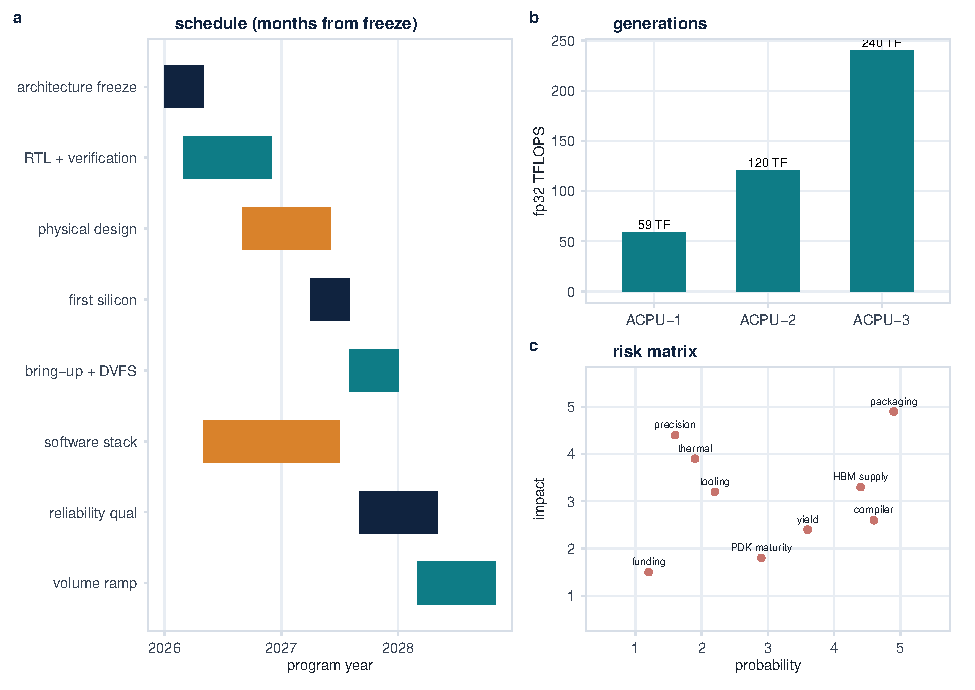
\includegraphics[width=\linewidth]{fig26_roadmap}
\caption{Roadmap. (a) 34-month programme from architecture freeze to volume ramp. (b) Three
generations. (c) Risk matrix; packaging, thermal and precision validation are the high-impact
items.}
\label{fig:roadmap}
\end{figure}

\subsection{Programme risks}
The risk matrix in Fig.~\ref{fig:roadmap}(c) ranks packaging and thermal as the highest-impact
items. Hybrid bonding of two 64 MB dies onto a 287.6 mm$^2$ compute die is the least mature step in
the flow; the fallback is a single 96 MB L3 die on the interposer, which costs 20\% of the L3
bandwidth and postpones the second-generation stack. HBM supply is a commercial risk rather than a
technical one. Precision validation on a full model is the highest technical risk with the lowest
mitigation cost: it is a software experiment that can run before tape-out.

\subsection{Conclusion}
This report specified a processor for atmospheric chaotic computation and evaluated it against the
machine that the field currently uses. The design is organised around three observations:
ensembles are the natural parallel dimension, stencils are memory problems, and forecast error is
chaotic rather than arithmetic. The resulting chip is small, air-cooled and cheap; it sustains
41.9 TFLOPS at 57 W, runs a 64-member 24-hour forecast in two minutes, and is projected to use
\ACRatioDay$\times$ less energy per forecast-and-analysis day than an H100 at comparable
wall-clock.

The number that matters is not the ratio itself. It is that the ratio survives the sensitivity
analysis, survives the idealised-GPU bound, and decomposes into mechanisms that can be measured on
real silicon. A 3.9$\times$ advantage at 100\% GPU utilisation is still a reason to build the
machine; a 9.3$\times$ advantage at realistic utilisation is a reason to build it now.

The next step is not another simulation. It is a two-week experiment on an H100 that runs the ten
kernels of Table~\ref{tab:kernels} at state-of-the-art efficiency and measures joules per
delivered forecast. That measurement would either validate the thesis or kill it, and either
outcome is worth more than a third decimal place in a projection.

\FloatBarrier
\appendix
\section{Instruction encoding and register map}\label{app:isa}

\begin{table}[h]
\centering\small
\caption{AVISA field encoding.}
\begin{tabular}{@{}llll@{}}
\toprule
Field & Bits & Position & Meaning\\
\midrule
opcode & 8 & 63--56 & operation (Table~\ref{tab:isa})\\
precision & 3 & 55--53 & 0 fp32, 1 fp16, 2 bf16, 3 fp8, 4 adaptive\\
vector mask & 3 & 52--50 & lane-group predicate (8 groups of 32 lanes)\\
rd & 5 & 49--45 & destination tile register\\
rs1 & 5 & 44--40 & first source tile register\\
rs2 & 5 & 39--35 & second source tile register\\
descriptor & 24 & 34--11 & stencil coefficients, halo offset, stride\\
member base & 8 & 10--3 & first ensemble member in the lane group\\
flags & 3 & 2--0 & Kahan, saturate, audit\\
\bottomrule
\end{tabular}
\end{table}

The tile register file has 32 registers of 256 lanes $\times$ 32 bits. The descriptor is interpreted
per opcode: for \code{STENCIL3D} it packs three 6-bit coefficients and a 6-bit halo mask; for
\code{DA.GAIN} it selects a localisation radius and a symmetry flag. There is no general addressing
mode; all memory references are offsets into the tile's 256 KB SRAM.

\section{Model parameters}\label{app:params}

\begin{table}[h]
\centering\small
\caption{Parameters of the pre-silicon model. The ``range'' column is the interval sampled in the
Monte-Carlo study.}
\begin{tabular}{@{}lrll@{}}
\toprule
Parameter & Value & Range & Source\\
\midrule
fp32 FMA energy & 0.42 pJ & $\pm$25\% & Horowitz 2014, scaled to 3 nm / 0.75 V\\
fp16 FMA energy & 0.24 pJ & $\pm$25\% & same, half-rate\\
fp8 MAC energy & 0.14 pJ & $\pm$25\% & same\\
SRAM read / write & 0.30 / 0.36 pJ per word & $\pm$25\% & published 3 nm SRAM\\
L3 (stacked) & 0.40 pJ/B & $\pm$25\% & hybrid-bonded SRAM estimate\\
HBM3E & 16.0 pJ/B & 9--24 & HBM3E datasheet, published PHY energy\\
Clock and PLL & 2.5 W & & design budget\\
Leakage & 4.0 W at 0.75 V, 85 $^\circ$C & & library estimate\\
GPU stencil efficiency & 0.30 & 0.15--0.60 & WRF / COSMO GPU studies\\
GPU power at load & 263 W on W1 & $\pm$30\% & H100 data sheet, load model\\
H100 peak fp32 / HBM & 67 TFLOPS / 3.35 TB/s & & data sheet\\
A100 peak fp32 / HBM & 19.5 TFLOPS / 2.04 TB/s & & data sheet\\
\bottomrule
\end{tabular}
\end{table}

\section{Reproducibility}\label{app:repro}

The complete results of this report are regenerated from the project root by the
following commands:
\begin{verbatim}
python3 sim/run_all.py            # 37 s -> results/*.json, *.csv, numbers.tex
Rscript figs/src/f01.R            # figure 01
Rscript figs/src/figs_data1.R     # data figures 12-17
Rscript figs/src/figs_data2.R     # data figures 08, 10, 21, 22, 25, 26
bash scripts/build-figures.sh     # schematic figures 02-07, 09, 11, 18-20, 23, 24
bash scripts/build-report.sh      # -> ACPU-1_Technical_Report.pdf
\end{verbatim}
The numerical experiments use fixed seeds, the PRNG is a PCG64 generator, and the model has no
randomness outside the Monte-Carlo study (which uses seed 42). The report is compiled with Tectonic (XeTeX) by \code{scripts/build-report.sh}. Figures are vector PDFs generated either by R (data) or by
Chromium (schematics); the UI figure is a set of screenshots of the running application.

\clearpage
\section{Acronyms}\label{app:acronyms}

\begin{multicols}{2}\small
\begin{itemize}[leftmargin=0pt,itemsep=0pt]
\item ACPU --- Atmospheric Calculation Processor Unit
\item AVT --- Atmospheric Vector Tile
\item AVISA --- ACPU Vector Instruction Set Architecture
\item BSPDN --- Backside Power Delivery Network
\item DA --- Data Assimilation
\item DVFS --- Dynamic Voltage and Frequency Scaling
\item EnKF --- Ensemble Kalman Filter
\item FIT --- Failures In Time (per $10^9$ device-hours)
\item FTLE --- Finite-Time Lyapunov Exponent
\item GAA --- Gate-All-Around
\item HBM --- High Bandwidth Memory
\item NoC --- Network-on-Chip
\item NWP --- Numerical Weather Prediction
\item SPPT --- Stochastically Perturbed Parameterisation Tendencies
\item SKEB --- Stochastic Kinetic Energy Backscatter
\item SRAM --- Static Random Access Memory
\end{itemize}
\end{multicols}

\renewcommand{\refname}{References}
\addcontentsline{toc}{section}{References}
\begin{thebibliography}{99}\small
\bibitem{lorenz1963} E. N. Lorenz, ``Deterministic nonperiodic flow,'' \emph{J. Atmos. Sci.}, vol. 20, no. 2, pp. 130--141, 1963.
\bibitem{lorenz1996} E. N. Lorenz, ``Predictability: a problem partly solved,'' in \emph{Proc. Seminar on Predictability}, ECMWF, 1996.
\bibitem{lorenz1998} E. N. Lorenz and K. A. Emanuel, ``Optimal sites for supplementary weather observations: simulation with a small model,'' \emph{J. Atmos. Sci.}, vol. 55, pp. 399--414, 1998.
\bibitem{kalnay2003} E. Kalnay, \emph{Atmospheric Modeling, Data Assimilation and Predictability}. Cambridge University Press, 2003.
\bibitem{evensen1994} G. Evensen, ``Sequential data assimilation with a nonlinear quasi-geostrophic model using Monte Carlo methods to forecast error statistics,'' \emph{J. Geophys. Res.}, vol. 99, no. C5, pp. 10143--10162, 1994.
\bibitem{bauer2015} P. Bauer, A. Thorpe and G. Brunet, ``The quiet revolution of numerical weather prediction,'' \emph{Nature}, vol. 525, pp. 47--55, 2015.
\bibitem{palmer2019} T. N. Palmer, ``Stochastic weather and climate models,'' \emph{Nature Reviews Physics}, vol. 1, pp. 463--471, 2019.
\bibitem{fuhrer2018} O. Fuhrer \emph{et al.}, ``Near-global climate simulation at 1 km resolution: establishing a performance baseline on 4888 GPUs with COSMO 5.0,'' \emph{Geosci. Model Dev.}, vol. 11, pp. 1665--1681, 2018.
\bibitem{wrf2019} W. C. Skamarock \emph{et al.}, ``A description of the Advanced Research WRF version 4,'' NCAR Tech. Note NCAR/TN-556+STR, 2019.
\bibitem{icon2015} G. Z\"angl \emph{et al.}, ``The ICON (ICOsahedral Non-hydrostatic) modelling framework of DWD and MPI-M,'' \emph{Geosci. Model Dev.}, vol. 8, pp. 3523--3542, 2015.
\bibitem{buizza1999} R. Buizza, M. Miller and T. N. Palmer, ``Stochastic representation of model uncertainties in the ECMWF ensemble prediction system,'' \emph{Q. J. R. Meteorol. Soc.}, vol. 125, pp. 2887--2908, 1999.
\bibitem{shutts2005} G. Shutts, ``A kinetic energy backscatter algorithm for use in ensemble prediction systems,'' \emph{Q. J. R. Meteorol. Soc.}, vol. 131, pp. 71--95, 2005.
\bibitem{salmon2011} J. K. Salmon, M. A. Moraes, R. O. Dror and D. E. Shaw, ``Parallel random numbers: as easy as 1, 2, 3,'' in \emph{Proc. SC'11}, 2011.
\bibitem{kahan1965} W. Kahan, ``Further remarks on reducing truncation errors,'' \emph{Comm. ACM}, vol. 8, no. 1, p. 40, 1965.
\bibitem{horowitz2014} M. Horowitz, ``Computing's energy problem (and what we can do about it),'' in \emph{IEEE ISSCC}, 2014, pp. 10--14.
\bibitem{jouppi2017} N. P. Jouppi \emph{et al.}, ``In-datacenter performance analysis of a tensor processing unit,'' in \emph{Proc. ISCA}, 2017, pp. 1--12.
\bibitem{h100} NVIDIA, \emph{H100 Tensor Core GPU Architecture}, whitepaper, 2022.
\bibitem{a100} NVIDIA, \emph{A100 Tensor Core GPU Architecture}, whitepaper, 2020.
\bibitem{hbm3} JEDEC, \emph{JESD238A: High Bandwidth Memory (HBM3) DRAM Standard}, 2023.
\bibitem{murphy1964} B. T. Murphy, ``Cost-size optima of monolithic integrated circuits,'' \emph{Proc. IEEE}, vol. 52, no. 12, pp. 1537--1545, 1964.
\bibitem{black1969} J. R. Black, ``Electromigration --- a brief survey and some recent results,'' \emph{IEEE Trans. Electron Devices}, vol. 16, no. 4, pp. 338--347, 1969.
\bibitem{weibull1951} W. Weibull, ``A statistical distribution function of wide applicability,'' \emph{J. Appl. Mech.}, vol. 18, pp. 293--297, 1951.
\bibitem{irds2023} International Roadmap for Devices and Systems, \emph{More Moore}, 2023 edition.
\bibitem{palmer2000} T. N. Palmer, ``Predicting uncertainty in forecasts of weather and climate,'' \emph{Rep. Prog. Phys.}, vol. 63, pp. 71--116, 2000.
\end{thebibliography}


\end{document}
